
\chapter{Capacity aware cartesian space trajectory planning}

\newcommand{\DD}[1]{\textcolor{teal}{[dd] #1}}
\newcommand{\redo}[1]{\todo[inline]{[redo] #1}}

With many promising collaborative robot applications in dynamical and unstructured human environments, there is an increasing need for real-time adaptable robot motion planning strategies. To reach the real-time execution times needed to ensure online adaptations, common techniques often make assumptions on robot's movement capacity considering them constant during the movement execution. However, robot's task-space movement capacity is state dependant and thus can evolve significantly during the execution of the movement.
To adapt to the real-time evolution of the robot's capacity, this paper proposes a method for real-time trajectory planning based on time-optimal Trapezoidal acceleration profile (TAP) trajectories. 
In each planning step, the robot's movement capacity is evaluated using an efficient approach for projecting the robot's kinematic limits in the trajectory direction, leveraging the convex polytope algebra.
\textcolor{red}{In addition to the robot's movement limits, the proposed method enables integrating task and environment-specific constraints as well.}

\textcolor{red}{
The method has been compared with state-of-the-art time-optimal joint space planning method TOPP-RA and traditional task-space TAP planning assuming constant movement capacity, given by the manufacturer. Results show that the proposed method has a comparable trajectory execution time as TOPP-RA, while exploiting the robot's movement capacity better and having lower tracking error than the traditional TAP approach. A mockup experiment is presented where the proposed method is used for collaborative waste sorting using a Franka Emika Panda robot, showing the efficiency of the approach in a real-world application.}

\section{Introduction}

The field of collaborative robotics has seen a unprecedented growth in recent years with the development of safer and cheaper robots with promising applications in industry, research, and even everyday life \cite{ajoudani2018progress}. However, as the complexity of the environments in which these robots operate increases, planning for robot trajectories becomes a significant challenge.  The robots need to adapt to changing environmental conditions and tasks, as well as the presence of humans. 
At the same time, in order to be safe, collaborative robots tend to be smaller and relatively limited in performance compared to more traditional industrial robots \cite{smu}. Therefore, it is becoming increasingly important to utilise the physical abilities of these robots fully in order for their applications to become viable, rather than investing in larger, more expensive industrial robots. 

%In addition, standard \textit{a priori} metrics of robot's physical abilities which underestimate them significantly do not scale well to these smaller robots, and new more precise and real-time capable solutions are needed to exploit their full potential.

When it comes to planning robot motions, the most common approach is to decouple path and trajectory planning \cite{Pardo1996}. First, the robot's geometric path is found, accomplishing certain task and potentially avoiding the obstacles in the environment. Then the optimal sequence of movements along this path is calculated in order to optimise certain criteria, the most common ones used in the literature being minimum energy, minimum jerk and minimum execution time. The criteria that aims to exploit full robot's movement capacity corresponds to finding the the time-optimal (minimum time) trajectories \cite{gasparetto2012trajectory}. 

Traditional time-optimal trajectory planning techniques, developed for industrial robots, find trajectories with the highest possible speeds, within robot's and task constraints, along predefined paths. Time-optimal algorithms, such as ones proposed Bobrow et al. \cite{bobrow1985time} and recently by Pham and Pham \cite{Pham2018}, assume full in advance knowledge about both robot's path and the the environment. However in collaborative scenarios, environment is often dynamic and conditions may change rapidly, requiring real-time changes in the trajectory and the task. To account for these changes the trajectory needs to be adapted in real-time, however time-optimal approaches have long execution times due to their computational complexity, making such implementations unpractical. 


\begin{figure}[!t]
    \centering
    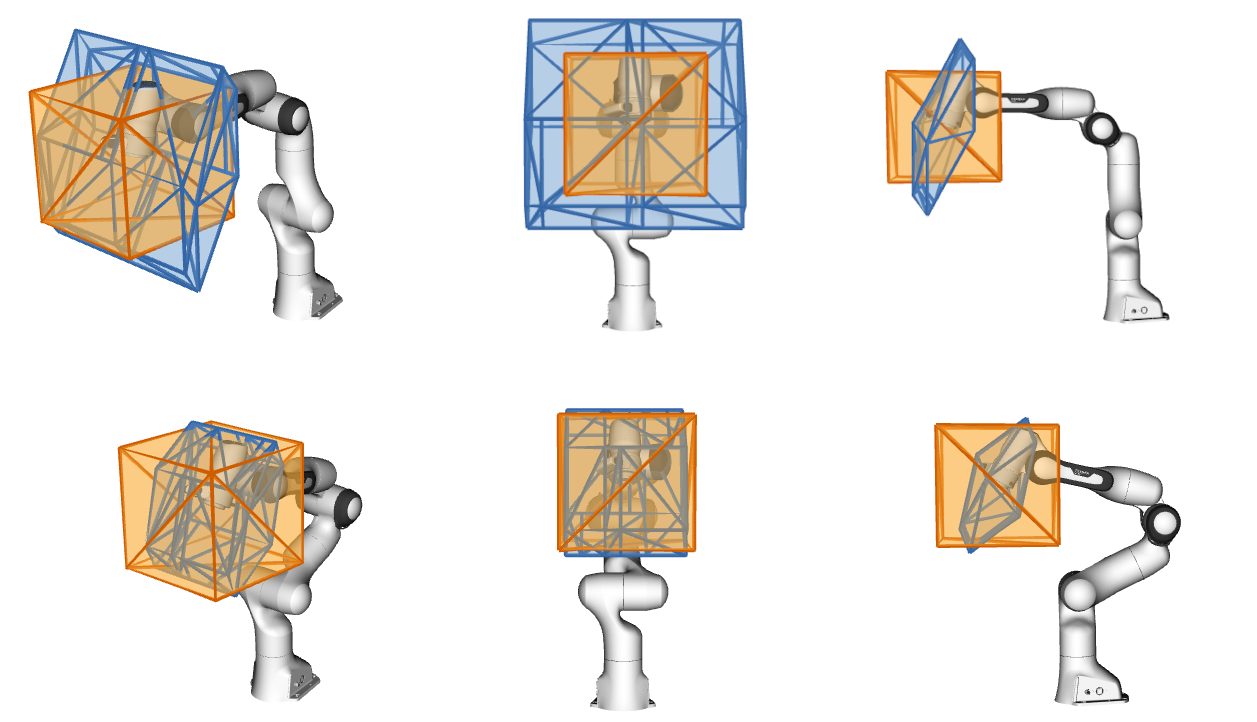
\includegraphics[width=0.8\linewidth]{img/comp_poly2.png}
    \caption{End-effector linear velocity limits as computed using the fixed Cartesian limits provided by the manufacturer (orange) and using an estimation based on the joint space velocity limits and the current configuration of the robot (blue) (scale: 1 m.s$^{-1}$/ 10 cm). The true robot's velocity capacity are in some directions higher and in the others significantly lower than the manufacturer's limits, depending on the configuration.}
    \label{fig:comp_cube_poly}
\end{figure}



On the other end of the spectrum, the real-time capable trajectory planning approaches often abstract the robot as a generator of ideal movements without accounting for its true capacity. With this simplification, they have short execution times and can quickly adapt to any changes in the robot's path, environment or the task itself. Such algorithms, as proposed by Macfarlane et al. \cite{Macfarlane2003}, Haschke et al. \cite{haschke2008line} or Svarny et al.\cite{Svarny2022}, are often based on S-curve trajectories \cite{FANG2019} with an appropriate order, producing smooth trajectories that respect a set of fixed velocity, acceleration, jerk and sometimes even snap (jerk derivative) limits enforced by the task and robot's capacity that are assumed to be constant \cite{modernrobotics}. However, robot's movement capacity is not constant and can vary significantly during the trajectory execution, therefore such approaches are not capable of fully exploiting the robot's capacity, resulting in trajectories that might underestimate or sometimes even overestimate its movement capacity. Figure \ref{fig:comp_cube_poly} shows an example of this effect on a Franka Emika Panda collaborative robot.


\textcolor{red}{
Several approaches have been proposed recently trying to bridge the gap proposing solutions that exploit robot's capacity while enabling different kinds of real-time adaptations. Palleschi et al.\cite{Palleschi2021} have used reactive real-time re-planning to adapt the pre-calculated time-optimal trajectory with the aim to guarantee human safety. Springer et al. \cite{dmp2014} have used dynamic motion primitives (DMP) to model an time-optimal point-to-point robot trajectory offline and then refined it during the real-time execution in order to account for changing target. Zhang et al. \cite{ZHANG2020} have proposed a real-time method for time-optimal trajectory planning based on a machine learning aided simplification of the robot's dynamical model resulting in more efficient calculation times. However, all these methods require a substantial degree of in advance computation in order to work properly.
}

\textcolor{red}{
A promising family of real-time solutions producing reactive and optimal trajectories without requiring \textit{a priori} knowledge about the desired path are the optimal control approaches such as Model predictive control (MPC). They have a potential to consider the robot's evolving movement capacity and adapt to the environmental changes in real-time \cite{torresalberto2022}\cite{Eckhoff2022}. However, they are still complex and challenging to implement as they often rely on nonlinear optimisation techniques \cite{kelff2021,Massaro2023}.}


In this paper, a real-time approach based on the time-optimal Trapezoidal acceleration profile (TAP) \cite{modernrobotics} planning in Cartesian space (CS) is proposed. The proposed approach evaluates the robot's movement capacity in real-time and plans the time-optimal TAP trajectory in each time-step. By leveraging the computational efficiency of TAP planning, the approach can create a real-time reactive trajectory generation while producing time-efficient trajectories that consider the robot's true capacity. The proposed approach provides a balance between reactive real-time adaptable solutions and time-optimal solutions, making it well-suited for dynamic environments where conditions change rapidly such as human-robot collaboration. 
Experimental results demonstrate the effectiveness of the proposed approach on a Franka Emika Panda collaborative robot, showing that the generated trajectories have comparable execution time (even shorter in some cases) as the state-of-the art offline time-optimal method TOPP-RA \cite{Pham2018}. Additionally the results confirm that the proposed method achieves faster and more precise trajectories than the standard TAP planning with fixed movement capacity given by the manufacturer. 

\todo{a sentence about waste sorting}

The paper gives an overview of the Cartesian space TAP planning and the description of the real-time planning strategy in section \ref{ch:tap}. A real-time method for robot's Cartesian kinematic capacity evaluation is described in section \ref{ch:capacity}. The experimental setup for assessing the performance of the proposed method on a Franka Emika Panda collaborative robot is given in section \ref{ch:setup}. A comparative study of the performance of the proposed algorithm with the time-optimal joint space and Cartesian space planning is given in \ref{ch:comp_study}. A mockup experiment of collaborative waste sorting is presented in \ref{ch:experiment_mockup}. Discussion about the limitations of the method is given in section \ref{ch:discussion}.


\section{Problem statement: Capacity aware trajectory planning }\label{ch:problem_statement}

Time-optimal trajectory planning requires a thorough understanding of the robot's movement capacity along the trajectory, which highly depends on its kinematics and joint actuation capabilities. Robot's actuation capabilities are usually expressed in the $n$-dimensional joints space, where its joint variables $\bm{q}$ are limited by its actuator limits $\mathcal{Q}$

\begin{equation}
\bm{q} \in \mathcal{Q}, \quad \bm{q}\in \bm{R}^n,
\end{equation}

However, as opposed to the the robot's joint actuation limits, the robot's path $\mathcal{T}$ is usually specified in the Cartesian (task) space.
\begin{equation}
\bm{x}(s) = \mathcal{T}(s) \in \bm{R}^6,\quad s\in\left[0,1\right]
\end{equation}
Where $s$ is the normalised position on the path in the range from $0$ to $1$. Then finding the minimal time trajectory $\mathcal{T}(t)$ corresponds to finding the optimal time evolution of the path variable $s(t)$ resulting in the mammal trajectory execution time, while respecting all the robots actuation limits $\mathcal{Q}$ \cite{modernrobotics}. 

However, to plan for such optimal task-space trajectory $\mathcal{T}(t)$, either the path $\mathcal{T}(s)$ needs to be transformed to the joint space or the robot's limits $\mathcal{Q}$ need to be transformed to the task space.
The transformation between the joint and task space is given through the robot's kinematics
\begin{equation}
f : \bm{q} \in R^n \to \bm{x}\in  R^6
\end{equation}

Most of the well known approaches to robot trajectory planning rely on transforming the robot's path $\mathcal{T}(s)$ to the joint space using robot's inverse kinematics $f^{-1}$, where it find the optimal time evolution of the joint variables $\bm{q}(t)$.
\begin{equation}
 \quad \bm{q}(t) = f^{-1}\left(~\mathcal{T}\left(s\left(t\right)\right)~\right), \quad\bm{q}(t) \in \mathcal{Q} 
\end{equation}
The main limitation of this approach is that the joint space is usually higher dimensional than Cartesian space ($n>6$), making the mapping $f^{-1}$ between the CS and JS not unique. In practice this means that there are multiple joint space paths that accomplish the same CS path. Each one of these JS path will have different properties which makes finding the optimal JS path a challenging problem of its own. Additionally, having chosen an appropriate JS path, the robot's redundant degrees of freedom are fixed even though they do not participate in movement generation, preventing it from executing other tasks and further limiting this approach.


\begin{figure}[!t]
    \centering 
    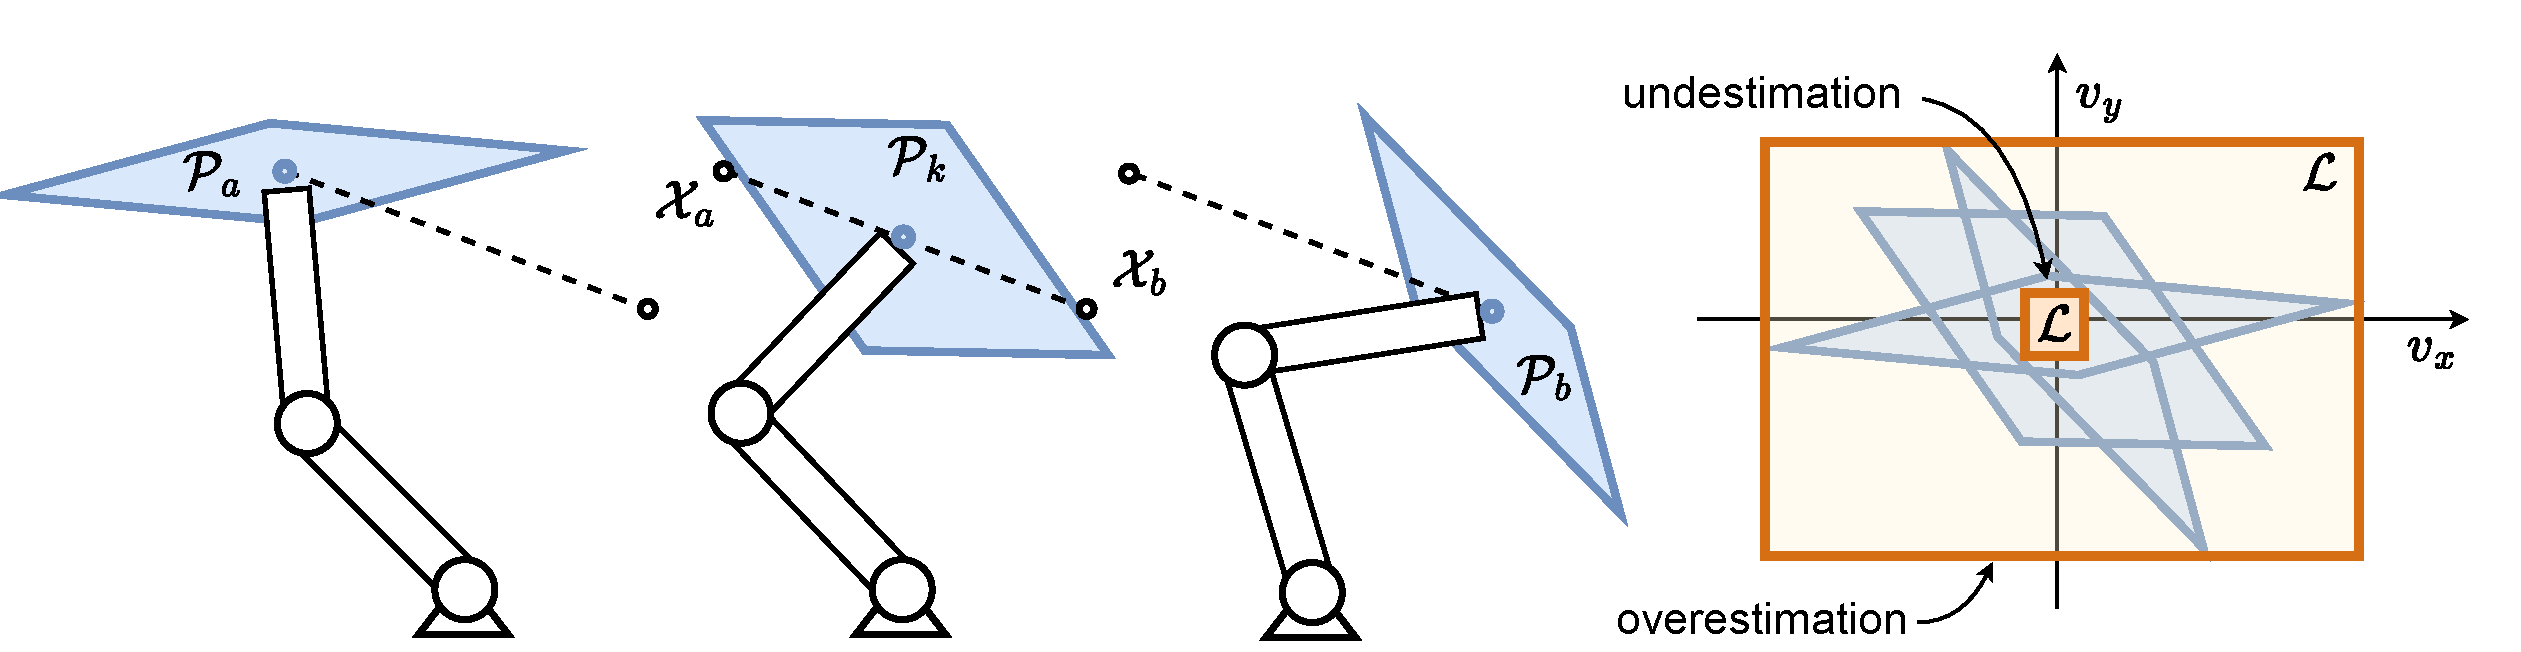
\includegraphics[width=\linewidth]{img/problem_statement_2link2.pdf}
    \caption{On the example of a 2 link planar robot, executing the trajectory form point $\mathcal{X}_a$ to $\mathcal{X}_b$. It's Cartesian space velocity capacity $\mathcal{P}(\bm{q})$ is shown in three different configurations. Finally the left plot shows the influence of the approximation strategy when representing these ever changing CS capacities with a fixed ranges $\mathcal{L}$. }
    \label{fig:2link}
\end{figure}


Complementary approach consists in transforming the robot's joint actuator limits $\mathcal{Q}$ to the Cartesian space and find the optimal time evolution of the Cartesian variable $\bm{x}(t)$
\begin{equation}
\bm{x}(t) = \mathcal{T}(s(t)) , \quad \bm{x}(t) \in f(\mathcal{Q})
\end{equation}
The resulting trajectory guarantees that $\bm{x}(t)$ is feasible given the joint limits $\mathcal{Q}$, without choosing the joint path $\bm{q}(t)$ directly. \textcolor{red}{The actual joint trajectory $\bm{q}(t)$ can then be found in real-time by using a lower level real-time control approaches such as inverse velocity kinematics solvers.\todo{qp paper here} Such approaches are capable of exploiting robot redundant degrees of freedom as well, there along the trajectory following, they can accomplish additional tasks such as avoiding singularities \cite{Cheng1995} or ensuring human safety\cite{joseph2020}. }

However, these new CS limits, obtained by projecting JS limits $\mathcal{Q}$ using robot's nonlinear kinematics $f(\mathcal{Q})$, have complex geometry forming robot configuration $\bm{q}$ dependant convex polytopes $\mathcal{P}(\bm{q}) = f(\mathcal{Q})$. Figure \ref{fig:2link} demonstrates an example of a two link planar robot executing a CS trajectory from pose $\mathcal{X}_a$ to $\mathcal{X}_b$. Its end-effector Cartesian velocity capacity polytope is shown in blue. It can be seen that its capacity varies substantially during the trajectory execution. In practice, to simplify the mapping $\mathcal{P}(\bm{q})$, the manufacturers often chose to transform it into fixed ranges of cartesian variables $\mathcal{P}(\bm{q}) \approx \mathcal{L}$. However, such choice typically requires a degree of under or over approximation of robot's abilities, as shown in the example on Figure \ref{fig:2link}. As a result, these limits $\mathcal{L}$ may not accurately represent the true limits of the robot's movement capacity $Q \neq f^{-1}(\mathcal{L})$. Figure \ref{fig:comp_cube_poly} shows the real world example of this discrepancy in the case of a Franka Emika Panda robot. 

In this paper an approach for trajectory planning in Cartesian space is proposed, able to fully exploit ever changing robot's movement capacity polytopes $\mathcal{P}(\bm{q})$ by efficiently evaluating them in the real-time and recalculating the optimal trajectory $\bm{x}(t)$ with updated limits $\mathcal{P}(\bm{q})$ in every step of the trajectory execution. In this way the proposed method is able to exploit robot's true movement capacity and at the same time it does not limit the robot's redundant degrees of freedom, which might be used for other tasks. 
\textcolor{red}{The proposed method is based on the assumption of straight line point to point motions in the Cartesian space. When considering straight line movements the task space becomes 1d and the limits $\mathcal{P}(\bm{q})$ become intervals. This simplification enables efficient and exact real-time evaluation of the movement capacity $\mathcal{P}(\bm{q})$ able to be executed online. }

%This limit calculation strategy is coupled with an efficient time-optimal planning technique based on the Trapezoidal acceleration profiles (TAP). 


\todo[inline]{straight lines - can be approximate any trajectory - way-points}


\section{Cartesian space trajectory planning accounting for evolving capacity}


\textcolor{red}{In order to enable a real-time adaptable planning of robot's Cartesian space motions, while exploiting its full motion capacity, this paper leverages the computational efficiency of the Trapezoidal acceleration profiles (TAP) or \textit{S-curve} velocity profiles \cite{ruckig}\cite{modernrobotics}\cite{scurve}. 
TAP is a classical approach to finding the Cartesian space time-optimal or minimum time\cite{Gasparetto2012} trajectories, assuming a set of fixed constants on Cartesian velocity $\dot{\bm{x}}$, acceleration $\ddot{\bm{x}}$ and jerk $\dddot{\bm{x}}$ \cite{Meckl1998,Garcia2017}. 
\begin{equation}
\begin{split}
 \dddot{\bm{x\!}}\! \in\![ \dddot{\bm{x}\!}_{min},  ~\dddot{\bm{x}\!}_{max}],&\quad
\ddot{\bm{x}} \! \in\! [\ddot{\bm{x}}_{min}, ~\ddot{\bm{x}}_{max}], \\ \dot{\bm{x}} \! \in\! [\dot{\bm{x}}_{min}&, ~\dot{\bm{x}}_{max}]
\end{split}
\label{eq:limits_cs}
\end{equation}
An example of a TAP profile is shown on Figure \ref{fig:tap_profile}.
}
\textcolor{red}{
However, as the robot's Cartesian space movement capacity is evolving in real-time with the changes in it's joint configuration $\bm{q}$, the limits (\ref{eq:limits_cs}) are no longer constant. To account for their changes, the proposed approach recalculates the optimal TAP trajectory in real-time, while updating the limits (\ref{eq:limits_cs}) in every planning step. Figure \ref{fig:replanning} shows the intuition of the proposed approach.
}

\textcolor{red}{ Section \ref{ch:tap} introduces the basics of the TAP planning followed by the section \ref{ch:update_cap} giving further insights in the real-time planning. }


\subsection{Trapezoidal acceleration profile basics}\label{ch:tap}

The robot's point to point path can be expresses as $\mathcal{T}(s)$, where $s\in\left[0,d\right]$ is a position on the path with a length $d$ \cite{Constantinescu2000,Pfeiffer1987}. A TAP trajectory results in a time optimal evolution of position $s(t)$, respecting the starting and end conditions 
\begin{equation}
    \dot{s}(0) = \dot{s}_{0} \quad \dot{s}(T) = \dot{s}_{T} \quad
    \ddot{s}(0) = \ddot{s}_{0} \quad \ddot{s}(T) = \ddot{s}_{T}
\end{equation}
as well as the limits on all its derivatives:
% \begin{equation}
% \begin{split}
%     \dot{s}  &\in  [\dot{s}_{min}, \dot{s}_{max}],\\
% \ddot{s} &\in [\ddot{s}_{min}, \ddot{s}_{max}],\\ 
% \dddot{s} &\in [\!\dddot{s}_{min}, \dddot{s}_{max}] 
% \end{split}\label{eq:s_limits}
% \end{equation}
\begin{equation}
\begin{split}
    \dot{s}\! \in\! [\dot{s}_{min}, \dot{s}_{max}], ~
\ddot{s}\!\in\! [\ddot{s}_{min}, \ddot{s}_{max}],~ 
\dddot{s}\!\in\! [\!\dddot{s\!}_{min}, \dddot{s\!}_{max}] 
\end{split}\label{eq:s_limits}
\end{equation}
where $T$ is the trajectory duration, $\dot{s}_{0}$ and $\ddot{s}_{0}$ represent the velocity and acceleration at the beginning of the path $\mathcal{T}(s)$, while the $\dot{s}_{T}$ and $\ddot{s}_{T}$ represent their final values at the end of the trajectory. One example of the TAP profile is shown on Figure \ref{fig:tap_profile}.


\begin{figure}
    \centering
    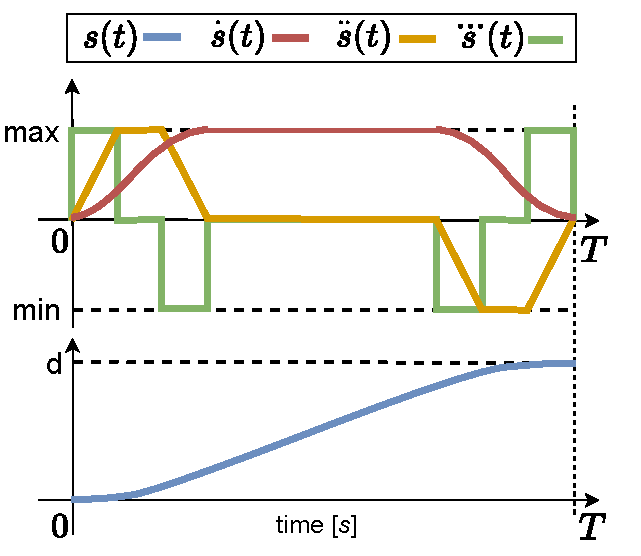
\includegraphics[width=\linewidth]{img/tap_profile.pdf}
    \caption{Trapezoidal acceleration profile example, all the initial and final conditions are set to 0.}
    \label{fig:tap_profile}
\end{figure}


TAP trajectory planned in CS results in time optimal evolution $\mathcal{X}(t)= \mathcal{T}\left(s(t)\right)$ of the Cartesian pose $\mathcal{X}(t)\in SE(3)$ of the desired robot's frame (ex. end-effector frame) with respect to the frame of interest (ex. inertial or robot base frame). When dealing with the geometric paths in CS, planning the robot's movement form a Cartesian pose $\mathcal{X}_a$ to $\mathcal{X}_b$, it is common to separate the translation $\mathcal{T}_t(s_t)$ and orientation $\mathcal{T}_r(s_r)$ component of the path $\mathcal{T}(s)$\cite{Bobrow1985}. The translation component of the path can then be expressed as:
\begin{equation}
    \mathcal{T}_t(s_t) = s_t \bm{u}_t, \quad s_t \in \left[0, ||\mathcal{X}_{b}^t - \mathcal{X}_{a}^t||_2\right]
\end{equation}
where $\mathcal{X}_{a}^t$ and $\mathcal{X}_{b}^t$ are the translation parts of the poses $\mathcal{X}_a$ and $\mathcal{X}_b$ and $\bm{u}_t$ is the unit vector pointing from $\mathcal{X}_{a}^t$ to $\mathcal{X}_{b}^t$. For the orientation, the common approach is to use the axis-angle representation of the rotation, and specify the difference in orientation between $\mathcal{X}_a$ and $\mathcal{X}_b$ as an angle $\theta$ around the axis $\bm{u}_{r}$. Then the geometric path corresponding to the orientation $\mathcal{T}_o(s_r)$ can be written as
\begin{equation}
    \mathcal{T}_r(s_r) = s_r \bm{u}_{r}, \quad s_r \in \left[0, \theta\right] 
\end{equation}
$\mathcal{T}_r(s_r)$ and $\mathcal{T}_t(s_t)$ represent a relative change in the orientation and translation over the course of the trajectory from the initial pose $\mathcal{X}_a$. Cartesian poses are commonly defined as homogeneous matrices in SE(3), therefore, the full desired Cartesian pose $\mathcal{X}(t)$ can be calculated using an homogeneous  transformation matrix $\Omega$, constructed from $\mathcal{T}_r$ and $\mathcal{T}_t$ 
\begin{equation}
    \mathcal{X}(t) = \mathcal{X}_a \Omega\left(\mathcal{T}_r(s_r), \mathcal{T}_t(s_t)\right)
\end{equation}
and optimal Cartesian velocity and acceleration can be found
\begin{equation}
    \dot{\bm{x}}(t)= \begin{bmatrix}\dot{s}_t(t) \bm{u}_t \\ \dot{s}_r( t) \bm{u}_r\end{bmatrix}, \quad 
    \ddot{\bm{x}}(t)= \begin{bmatrix}\ddot{s}_t(t) \bm{u}_t \\ \ddot{s}_r(t) \bm{u}_r\end{bmatrix}
\end{equation}
Cartesian $\dot{\bm{x}}$, acceleration $\ddot{\bm{x}}$ and jerk $\dddot{\bm{x}}$ limits (\ref{eq:limits_cs}) can then be projected on the path transforming them to limits on the trajectory variables $s_r(t)$ and $s_t(t)$, using vectors $\bm{c}_t = [\bm{u}_t^T, \bm{0}_{3\times 1}]^T$ and $\bm{c}_r =[\bm{0}_{3\times 1}, \bm{u}_r^T]^T$
\begin{equation}
\begin{split}
\bm{c}^T_i\dddot{\bm{x}}_{min} \leq \dddot{\bm{s}}_i(t)&  \leq  \bm{c}^T_i\dddot{\bm{x}}_{max} \\
\bm{c}^T_i\ddot{\bm{x}}_{min} \leq \ddot{\bm{s}}_i(t)&  \leq \bm{c}^T_i\ddot{\bm{x}}_{max} \\
\bm{c}^T_i\dot{\bm{x}}_{min} \leq \dot{\bm{s}}_i(t)&  \leq \bm{c}^T_i\dot{\bm{x}}_{max}\\
 \end{split} \label{eq:limits_s_cs}
\end{equation}
% \begin{equation}
% \begin{split}
% \dddot{\bm{s}}_i&  \in [ \bm{c}^T_i\dddot{\bm{x}}_{min},  ~\bm{c}^T_i\dddot{\bm{x}}_{max} ]\\
% \ddot{\bm{s}}_i&  \in [ \bm{c}^T_i\ddot{\bm{x}}_{min},  ~\bm{c}^T_i\ddot{\bm{x}}_{max} ]\\
% \dot{\bm{s}}_i&  \in [ \bm{c}^T_i\dot{\bm{x}}_{min},  ~\bm{c}^T_i\ddt{\bm{x}}_{max} ]\\
%  \end{split} \label{eq:limits_s_cs}
% \end{equation}
% \begin{equation}
% \begin{split}
% &\dddot{\bm{s}}_i  \in [ \bm{c}^T_i\dddot{\bm{x}}_{min},  ~\bm{c}^T_i\dddot{\bm{x}}_{max} ],
% \ddot{\bm{s}}_i  \in [ \bm{c}^T_i\ddot{\bm{x}}_{min},  ~\bm{c}^T_i\ddot{\bm{x}}_{max} ]\\
% &\qquad\qquad\qquad \dot{\bm{s}}_i  \in [ \bm{c}^T_i\dot{\bm{x}}_{min},  ~\bm{c}^T_i\dot{\bm{x}}_{max} ]\\
%  \end{split}\label{eq:limits_s_cs}
% \end{equation}
where $i$ is either the translation $t$ or the orientation $o$.

%\DD{Etre plus précsis dans les equations qui melangent translation et orientation, $c_i$ semble être de dimension 3}

Finally, once both translation and orientation TAP trajectories are found resulting in optimal $s_r(t)$ and $s_t(t)$, to synchronise the two movements, their time duration is matched, making both trajectories last the same time $T$, the time taken by the longer of the two trajectories $T = \max\{T_r,T_t\}$. 

\subsection{Allowing for real-time updates of Task space capacity}
\label{ch:update_cap}


\begin{figure}[t]
    \centering
    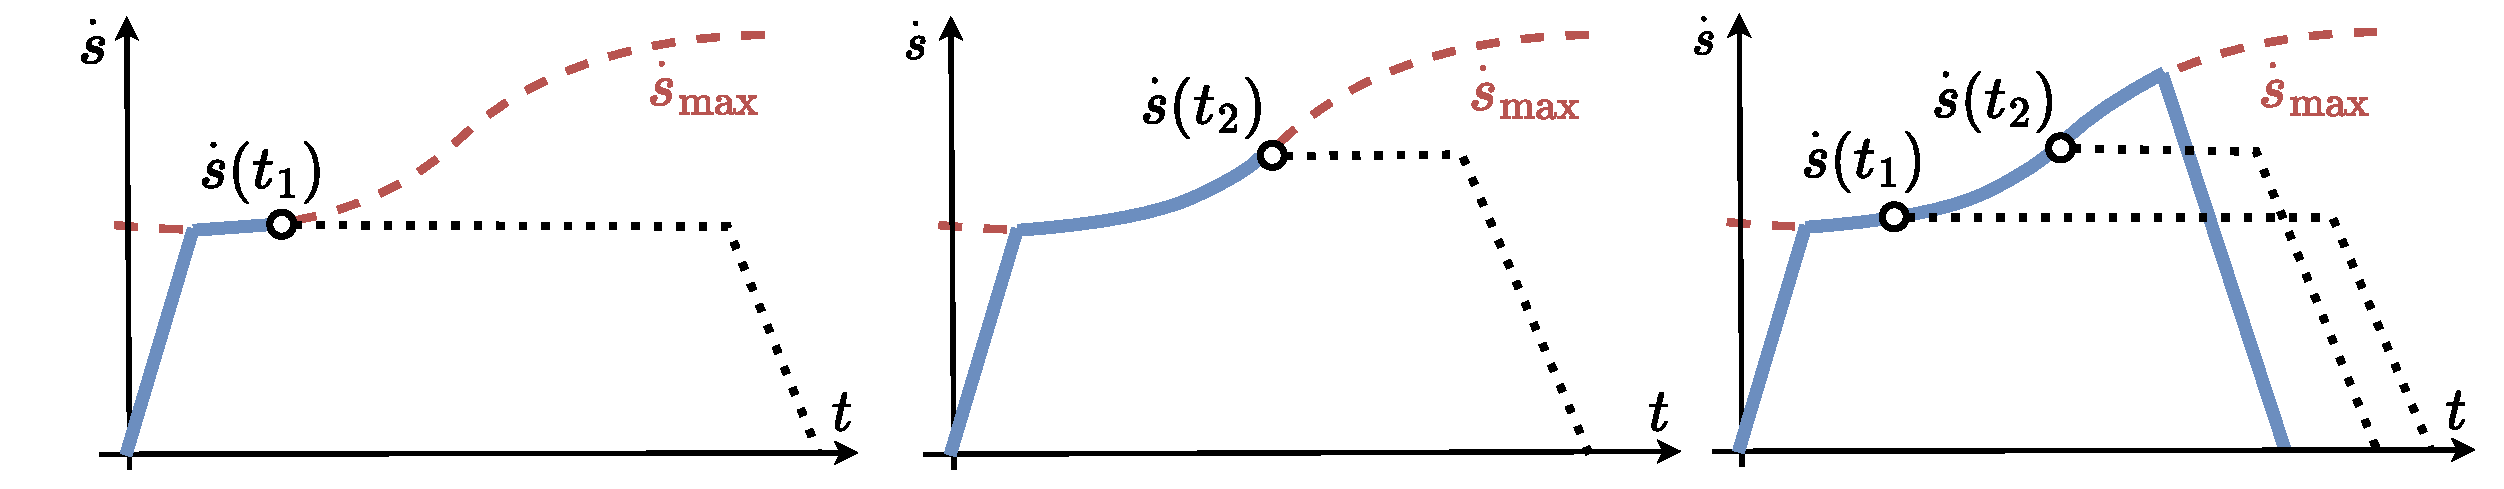
\includegraphics[width=\linewidth]{img/tap_replanning3.pdf}
    % 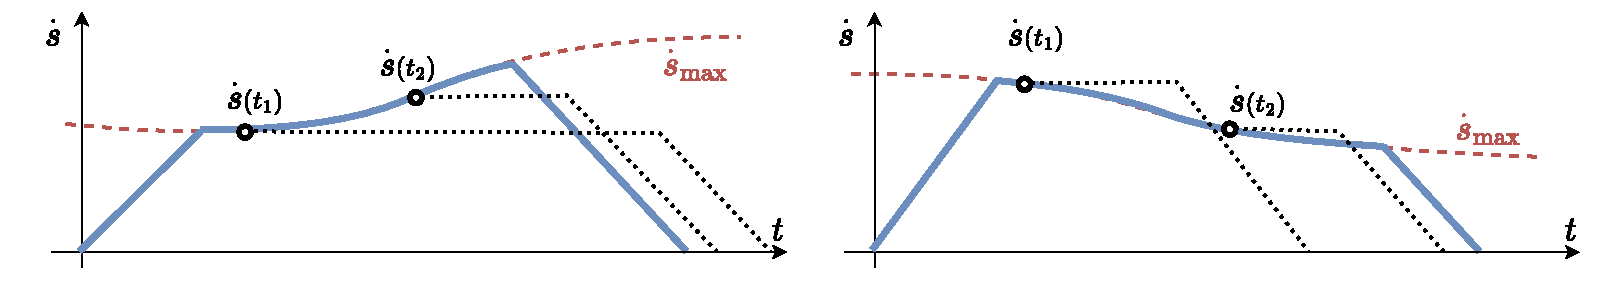
\includegraphics[width=\linewidth]{img/ICRA2023.drawio (25).pdf}
    \caption{Velocity curve, updated in the real time with instantaneous maximal values. At each time-step $t_k$ during the trajectory execution (ex. $t_1$ and $t_2$) the TAP planning calculates the remaining trajectory considering that maximal velocity $\dot{s}_{max}$ constant till the end of the movement (black dotted lines). As the maximal velocity $\dot{s}_{max}$ increases during the trajectory execution (red dashed line), the final trajectory duration is considerably shorter. }
    \label{fig:replanning}
\end{figure}

The inherent challenge of planning the robot motion in the Cartesian space is that its Cartesian kinematic limits (\ref{eq:limits_cs}) are configuration dependant, and over the course of the trajectory the robot's Cartesian capacity can change significantly. Therefore, no set of fixed Cartesian limits as defined in (\ref{eq:limits_cs}) will be able to exploit the robot's full movement capabilities.  

To address the issue of constantly changing kinematic limits (\ref{eq:s_limits}), during robot trajectory execution, a real-time replanning strategy is proposed. This approach involves evaluating the jerk $\dddot{s}$, acceleration $\ddot{s}$ and velocity $\dot{s}$ limits at each step of the trajectory execution based on its current movement capabilities. These updated limits are then considered constant until the end of the movement and used in conjunction with the TAP algorithm to calculate the time-optimal profile of the remaining trajectory.  
%Ultimately, this strategy enables the robot to follow the same path from the start to the end pose, but at a slower or faster pace based on its current capacity.

For a given moment in time $t_k$ and robot's position on the trajectory $s_t(t_k),s_r(t_k)$, the remaining length of the 
geometric path to the target position can be calculated as $d_k = s_{t,T} - s_t(t_k)$ and the remaining angle of rotation $\theta_k\!=\!s_{r,T}\! - \!s_r(t_k)$. Then the initial conditions for the new planning execution can be updated 
\begin{equation}
\begin{split}
    s_t \in [0, d_k], \quad \dot{s}_{t,0} = \dot{s}_t(t_k), \quad \ddot{s}_{t,0} = \ddot{s}_t(t_k),\\ 
    s_r \in [0 , \theta_k], \quad \dot{s}_{r,0} = \dot{s}_r(t_k), \quad \ddot{s}_{r,0} = \ddot{s}_r(t_k)
\end{split}\label{eq:rt_init}
\end{equation}

Finally, an updated TAP trajectory can then be calculated for the translation $s_t(t)$ and the orientation $s_r(t)$, resulting in an optimal robot trajectory given the updated robot's limits (\ref{eq:s_limits}) and the initial conditions (\ref{eq:rt_init}). 
The assumption of constant limits (\ref{eq:s_limits}) for the duration of the remaining trajectory is a simplification that might not hold true in practice, as the robot's movement capacity can change significantly over time. However, this issue is addressed through real-time planning, which constantly updates the plan using the latest information on the robot's current ability. The TAP planning algorithm is well-suited for this approach, as it is highly efficient in computing optimal trajectories in real-time. 

An example of the generated velocity $\dot{s}$ profile using real-time TAP replanning, with constantly changing limits $\dot{s}_{max}$, is shown on Figure \ref{fig:replanning}. 

\section{Real-time robot's capacity evaluation}
\label{ch:capacity}

Robot's joint actuator limits are usually given by the manufacturer as ranges of the feasible joint positions $\bm{q}$, velocity $\bm{q}$, acceleration $\dot{\bm{q}}$ and jerk $\ddot{\bm{q}}$
\begin{equation}
\begin{split}
\dddot{\bm{q}} \in [ \dddot{\bm{q}}_{min}, \dddot{\bm{q}}_{max}] ,&~\ddot{\bm{q}} \in [\ddot{\bm{q}}_{min},  \ddot{\bm{q}}_{max}],\\ 
\dot{\bm{q}} \in [\dot{\bm{q}}_{min},  \dot{\bm{q}}_{max}],&~{\bm{q}} \in [{\bm{q}}_{min},  {\bm{q}}_{max}]
\end{split}
\label{eq:kin_limits}
\end{equation}

The mapping between the robot's joint space and Cartesian space velocity, acceleration and jerk for a certain fixed frame of interest (ex. end-effector frame) is nonlinear and dependant on $\bm{q}$, $\{\bm{q},\dot{\bm{q}}\}$ and $\{\bm{q},\dot{\bm{q}},\ddot{\bm{q}}\}$ respectively 
\begin{equation}
\begin{split}
\dot{\bm{x}}&= J(\bm{q})\dot{\bm{q}}\\
\ddot{\bm{x}}&= J(\bm{q})\ddot{\bm{q}} + \dot{J}(\bm{q},\dot{\bm{q}})\dot{\bm{q}}\\
\dddot{\bm{x}}&= J(\bm{q})\dddot{\bm{q}} + 2\dot{J}(\bm{q},\dot{\bm{q}})\ddot{\bm{q}} + \ddot{J}(\bm{q},\dot{\bm{q}},\ddot{\bm{q}})\dot{\bm{q}}\\
 \end{split} \label{eq:js_to_cs_vaj}
\end{equation}
For a certain joint configuration $\bm{q}$, the joint velocity $\dot{\bm{q}}$, acceleration $\ddot{\bm{q}}$ and jerk $\dddot{\bm{q}}$ are mapped to Cartesian space using the Jacobian matrix $J(\bm{q})$ and its time derivatives $\dot{J}(\bm{q},\dot{\bm{q}})$ and  $\ddot{J}(\bm{q},\dot{\bm{q}},\ddot{\bm{q}})$. 

Joint space kinematic limits (\ref{eq:kin_limits}) are expressed in a form of an interval for each of the robot's $n$ joints (degrees of freedom), forming $n$-dimensional hypercubes. For any given robot state $\bm{q}_k,\dot{\bm{q}}_k,\ddot{\bm{q}}_k$, CS kinematic limits can be calculated by projecting these JS $n$-dimensional hypercubes (\ref{eq:kin_limits}) into the $m$-dimensional CS using the expressions (\ref{eq:js_to_cs_vaj}). The resulting CS limits will have a form of convex polytopes. 

For a certain robot pose $\bm{q}_k$ the convex polytope $\mathcal{P}_v$ of achievable CS velocities $\dot{\bm{x}}$ can be expressed as
\begin{equation}
    \mathcal{P}_v = \left\{ \dot{\bm{x}}\in\mathbf{R}^m | \dot{\bm{x}}=J(\bm{q}_k)\dot{\bm{q}}\! +\! \bm{v}_b, ~ \dot{\bm{q}}\in \left[\dot{\bm{q}}_{min}, \dot{\bm{q}}_{max} \right] \right\}
    \label{eq:vel_poly}
\end{equation}
where $\bm{v}_b$ is a bias vector $\bm{v}_b\!=\!\bm{0}_{m\times 1}$. The convex polytopes $\mathcal{P}_a$ and $\mathcal{P}_j$ of achievable CS acceleration $\ddot{\bm{x}}$ and jerk $\dddot{\bm{x}}$ have a form
\begin{equation}
\begin{split}
    \mathcal{P}_a \!&=\! \left\{ \ddot{\bm{x}}\in\mathbf{R}^m | \ddot{\bm{x}}=J(\bm{q}_k)\ddot{\bm{q}}\! +\! \bm{a}_b, ~ \ddot{\bm{q}}\in \left[\ddot{\bm{q}}_{min}, \ddot{\bm{q}}_{max} \right] \right\}\\
    \mathcal{P}_j\!&=\! \left\{ \dddot{\bm{x}}\!\in\mathbf{R}^m | \dddot{\bm{x}}\!=\!J(\bm{q}_k)\dddot{\bm{q}}\! \!+\!\bm{j}_b, ~ \!\dddot{\bm{q\!}}\!\in \left[\!\dddot{\bm{q\!}}_{min}, \dddot{\bm{q\!}}_{max} \right] \right\}
\end{split}\label{eq:jerk_acc_poly}
\end{equation}
where $\bm{a}_b$ and $\bm{j}_b$ are the bias acceleration and jerk produced by the effect of current joint velocity $\dot{\bm{q}}_k$ and acceleration $\ddot{\bm{q}}_k$ 
\begin{equation}
\begin{split}
\bm{a}_b&= \dot{J}(\bm{q}_k,\dot{\bm{q}}_k)\dot{\bm{q}}_k\\
\bm{j}_b&= 2\dot{J}(\bm{q}_k,\dot{\bm{q}}_k)\ddot{\bm{q}}_k + \ddot{J}(\bm{q}_k,\dot{\bm{q}}_k,\ddot{\bm{q}}_k)\dot{\bm{q}}_k\\
 \end{split} \label{eq:bias_terms}
\end{equation}
Additionally, as the $\bm{j}_b$ term produced by the second derivative of the Jacobian matrix $\ddot{J}(\bm{q}_k,\dot{\bm{q}}_k,\ddot{\bm{q}}_k)\dot{\bm{q}}_k$ will produce relatively small effects on final value of $\bm{j}_b$, in the case of this paper it is neglected $\ddot{J}(\bm{q}_k,\dot{\bm{q}}_k,\ddot{\bm{q}}_k)\dot{\bm{q}}_k \approx 0$. Finally, the achievable CS velocity, acceleration and jerk, given current robot state $\bm{q}_k,\dot{\bm{q}}_k,\ddot{\bm{q}}_k$ can be expressed as
\begin{equation}
    \dot{\bm{x}}\in \mathcal{P}_v, \quad \ddot{\bm{x}}\in \mathcal{P}_a, \quad \dddot{\bm{x}}\in \mathcal{P}_j\label{eq:limits_poly}
\end{equation}

Polytope definition (\ref{eq:vel_poly}) and (\ref{eq:jerk_acc_poly}) is an overestimation of the robot's real capacity as the joint kinematic limits are considered independent, which is not usually the case (ex. reaching $\dot{\bm{q}}_{max}$ in some configuration might violate joint acceleration $\ddot{\bm{q}}_{max}$  or jerk $\dddot{\bm{q}}_{max}$ limits). However, these limits can directly be used for TAP planning, as it inherently accounts for this issue and finds the trajectory respecting all the set constraints at the same time. 

\subsection{Finding Cartesian limits in trajectory direction}
\label{ch:capacity_lp}

Given a $m$-dimensional Cartesian space vector $\bm{c}$, pointing in the direction of the trajectory, the trajectory $m\!-\!1$ dimensional normal space can be found using the singular value decomposition (SVD)
\begin{equation}
    \bm{c} = U\Sigma V^T \quad V = \left[ V_1, ~ V_2\right], \quad V_2 \in \mathbf{R}^{m \times (m-1)}  
\end{equation}
where matrix $V_2$ represents the projector to the \textit{null-space} of $\bm{c}$\cite{klema_singular_1980}. Columns $\bm{n}_i$ of $V_2=\left[\bm{n}_1,~ \ldots~, \bm{n}_{m-1} \right]$ are an orthonormal base of the $m\!-\!1$ dimensional space normal to the vector $\bm{c}$, or in other words $V_2^T\bm{c} = \bm{0}$

With the known trajectory direction $\bm{c}$ and the trajectory normal space $V_2$, the maximal value of the Cartesian variable $\bm{y} \in\mathbf{R}^m$, in the trajectory direction $\bm{c}$, within its range expressed as a convex polytope $\mathcal{P}_y$, can be found by solving the Linear programming (LP) problem\cite{vajda_gass_1964}
% \begin{equation}
% \begin{split}
%     \max_{\bm{y}} ~c^T \bm{y}&\\
%     s.t. ~ V_2^T\bm{y} &= \bm{0}\\
%     \bm{y}&\in \mathcal{P}_y
% \end{split}\label{eq:lp_general}
% \end{equation}
\begin{equation}
\begin{split}
    \max_{\bm{y}} ~c^T \bm{y}& \\
    s.t. ~ V_2^T\bm{y} &= \bm{0}, \\
    \bm{y}&\in \mathcal{P}_y
\end{split}\label{eq:lp_general}
\end{equation}
whereas the minimum can be found by minimising it\cite{Skuric2022}.

% \begin{figure}
%     \centering
%     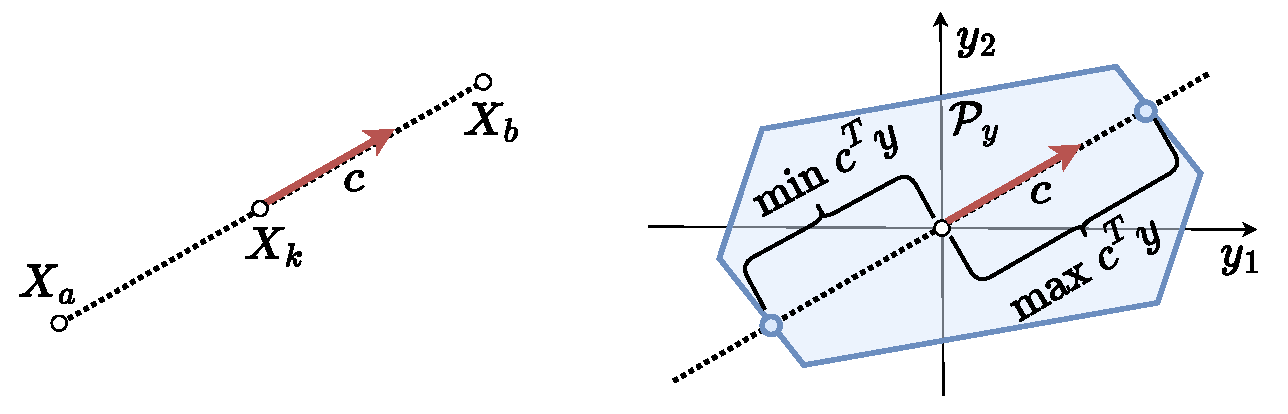
\includegraphics[width=0.7\linewidth]{img/dirs.pdf}
%     \caption{Can be removed}
%     \label{fig:normal_lp}
% \end{figure}


By substituting the generic Cartesian variable $\bm{y}$ with Cartesian velocity $\dot{\bm{x}}$, acceleration $\ddot{\bm{x}}$ and jerk $\dddot{\bm{x}}$ and its polytope $\mathcal{P}_y$  with their respective polytopic limits (\ref{eq:limits_poly}), LP formulation (\ref{eq:lp_general}) can be directly used to calculate the limits of the velocity $\dot{s}$, acceleration $\ddot{s}$ and jerk $\dddot{s}$ in the trajectory direction $\bm{c}$.  

When searching for maximal Cartesian velocity $\dot{s}_{max}$, assuming known robot configuration $\bm{q}_k$ and trajectory direction vector $\bm{c}$, the Cartesian velocity along the trajectory $\dot{s}$ can be calculated as a projection of the Cartesian velocity $\dot{\bm{x}}$ 
\begin{equation}
    \dot{s} = \bm{c}^T\dot{\bm{x}}= \bm{c}^TJ(\bm{q}_k)\dot{\bm{q}} = \bm{c}^TJ(\bm{q}_k)\dot{\bm{q}} + \bm{c}^T\bm{v}_b
\end{equation}
where $\bm{v}_b \in \bm{R}^6$ is zero vector. Substituting this relationship into the LP formulation (\ref{eq:lp_general}) yields 
\begin{equation}
\begin{split}
    \dot{s}_{max} = \max_{\dot{\bm{q}}} \bm{c}^TJ(\bm{q}_k)\dot{\bm{q}} &+ \bm{c}^T\bm{v}_b  \\
    s.t.\quad V_2^TJ(\bm{q}_k)\dot{\bm{q}} &= - V_2^T\bm{v}_b, \\
    \dot{\bm{q}}&\in [\dot{\bm{q}}_{min}, \dot{\bm{q}}_{max}]
\end{split}\label{eq:lp_vel_max}
\end{equation}
The equivalent LP expressions for finding the maximal acceleration $\ddot{s}$ and jerk $\dddot{s}$ are obtained by substituting $\dot{\bm{q}}$ and $\bm{v}_b$ with  $\ddot{\bm{q}}$, $\bm{a}_b$ and $\dddot{\bm{q}}$, $\bm{j}_b$. The minimal values are found by minimising the same problem.

\subsection{Task induced cartesian limits}

In many cases however, when planning for CS movement, the task requires limiting maximal cartesian velocity, acceleration and jerk. For example, when executing trajectories in the human vicinity, it is common practice to limit the robot's CS velocity $\dot{\bm{x}}$ to minimise the potential impact forces due to the robot's moment of inertia \cite{smu} and kinetic energy \cite{joseph2020}.
On the other hand, when designing trajectories of robotic manipulation of liquids, in order to prevent its sloshing or spilling, translation acceleration $\ddot{\bm{x}}$ continuity needs to be ensured \cite{moriello2018}, which in term corresponds to introducing CS jerk $\dddot{\bm{x}}$ limits.

Therefore, if an additional task specific limit of a CS variable $\bm{y}$ (velocity, acceleration or jerk) is required that can be expressed as an interval
\begin{equation}
\bm{y}\in  &[\bm{y}_{min},\bm{y}_{max}]\label{eq:limits_cs_additional}
\end{equation}
or more generally in a form of polytope defined by a set of inequality constraints
\begin{equation}
\mathcal{C} = \left\{ \bm{y} ~|~ A \bm{y} \leq \bm{b} \right\}
\label{eq:cartesian_polytope_additional}
\end{equation}
Then the LP problem (\ref{eq:lp_general}) can be extended to account for the polytope (\ref{eq:cartesian_polytope_additional})
\begin{equation}
\begin{split}
    \max_{\bm{y}} ~c^T \bm{y}& \\
    s.t. ~ V_2^T\bm{y} &= \bm{0}, \\
    \bm{y}&\in \mathcal{P}_y \cap \mathcal{C}
\end{split}\label{eq:lp_general_additional}
\end{equation}
\todo[inline]{I could maybe add inequality constraints rather than put this intersection $\mathcal{P}_y \cap \mathcal{C}$}

Following the same example of maximal velocity $\dot{s}_{max}$ along the trajectory from (\ref{eq:lp_vel_max}), if an additional CS limits are imposed by the task 

\begin{equation}
\mathcal{C}_v = \left\{ \dot{\bm{x}} ~|~ A \dot{\bm{x}} \leq \bm{b} \right\}
\label{eq:example_vel_poly}
\end{equation}
the maximal velocity $\dot{s}_{max}$ along the trajectory that respects both task constraint (\ref{eq:example_vel_poly}) and robot's instantaneous movement capacity (\ref{eq:vel_poly}), can be found by extending the LP formulation (\ref{eq:lp_vel_max})
\begin{equation}
\begin{split}
    \dot{s}_{max} = \max_{\dot{\bm{q}}} \bm{c}^TJ(\bm{q}_k)\dot{\bm{q}} &+ \bm{c}^T\bm{v}_b  \\
    s.t.\quad V_2^TJ(\bm{q}_k)\dot{\bm{q}} &= - V_2^T\bm{v}_b, \\
    AJ(\bm{q}_k)\dot{\bm{q}} &\leq \bm{b} - A\bm{v}_b, \\
    \dot{\bm{q}}&\in [\dot{\bm{q}}_{min}, \dot{\bm{q}}_{max}]
\end{split}\label{eq:lp_vel_max_additional}
\end{equation}

The lower limit $\dot{s}_{min}$ can be found by minimising the same problem.

\todo[inline]{Should I talk about acceleration and jerk?}

\subsection{Scaling robot's Cartesian limits}
\todo[inline]{optional}
When it comes to planning robot trajectories, it is a common practice to consider only a part (certain percentage) of the specified robot limits. This is partially due to the fact that more dynamic robot movements require higher actuation capacity and leave less margin to account for potential tracking error, in many cases resulting in impaired tracking performance. Additionally, robot movement with higher velocity is associated with longer stopping time and higher potential impact momentum \cite{smu}, therefore scaling strategies can be used to adapt robot's velocity in order to improve the safety. 
\todo[inline]{repetition of the safety applications here}

If the robot's CS kinematic limits are considered constant and if they are specified as (\ref{eq:limits_cs}), the simplest form of scaling can be done by multiplying the specified limits with scalar factors $\alpha_v,\alpha_a,\alpha_j\in[0,1]$.
\begin{equation}
\begin{split}
\dot{\bm{x}}&\in  [\alpha_v\dot{\bm{x}}_{min},\alpha_v\dot{\bm{x}}_{max}] \\
\ddot{\bm{x}}&\in  [\alpha_a\ddot{\bm{x}}_{min},\alpha_a\ddot{\bm{x}}_{max}] \\
\dddot{\bm{x}}&\in  [\alpha_j\dddot{\bm{x}}_{min},\alpha_j\dddot{\bm{x}}_{max}] \\
 \end{split} \label{eq:limits_cs_alpha}
\end{equation}
% \begin{equation}
% \begin{split}
% &\dot{\bm{x}} \in  [\alpha_v\dot{\bm{x}}_{min},\alpha_v\dot{\bm{x}}_{max}], \; 
% \ddot{\bm{x}} \in  [\alpha_a\ddot{\bm{x}}_{min},\alpha_a\ddot{\bm{x}}_{max}], \\
% &\qquad\qquad\dddot{\bm{x}} \in  [\alpha_j\dddot{\bm{x}}_{min},\alpha_j\dddot{\bm{x}}_{max}] 
% \end{split}
%  \label{eq:limits_cs_alpha}
% \end{equation}
allowing the robots velocity $\dot{\bm{x}}$, acceleration $\ddot{\bm{x}}$ and jerk $\dddot{\bm{x}}$ not to exceed certain percentage of the specified limits. 

However, if the robot's CS kinematic capacity is not considered constant but a result of the robot's current configuration $\bm{q}$ and its JS kinematic limits, then the scaling using the scalars $\alpha_v,\alpha_a,\alpha_j\in[0,1]$ can done in the joint space
\begin{equation}
\begin{split}
\dot{\bm{q}}&\in  [\alpha_v\dot{\bm{q}}_{min},\alpha_v\dot{\bm{q}}_{max}] \\
\ddot{\bm{q}}&\in  [\alpha_a\ddot{\bm{q}}_{min},\alpha_a\ddot{\bm{q}}_{max}] \\
\dddot{\bm{q}}&\in  [\alpha_j\dddot{\bm{q}}_{min},\alpha_j\dddot{\bm{q}}_{max}] \\
 \end{split} \label{eq:limits_cs_alpha}
\end{equation}
% \begin{equation}
% \begin{split}
% &\dot{\bm{q}}\in  [\alpha_v\dot{\bm{q}}_{min},\alpha_v\dot{\bm{q}}_{max}], 
% \ddot{\bm{q}}\in  [\alpha_a\ddot{\bm{q}}_{min},\alpha_a\ddot{\bm{q}}_{max}],\\
% &\qquad\qquad\dddot{\bm{q}}\in  [\alpha_j\dddot{\bm{q}}_{min},\alpha_j\dddot{\bm{q}}_{max}]
% \end{split}\label{eq:limits_cs_alpha}
% \end{equation}
These new modulated JS limits can then be used to calculate the polytopes $\mathcal{P}_v$,$\mathcal{P}_a$ and $\mathcal{P}_j$ using equations (\ref{eq:vel_poly}-\ref{eq:jerk_acc_poly}), and in term scale the resulting Cartesian robot limits (\ref{eq:limits_poly}).


\subsection{Real-time TAP planning undesirable effects}
\label{ch:heuristics}

\begin{figure}[tb!]
    \centering
    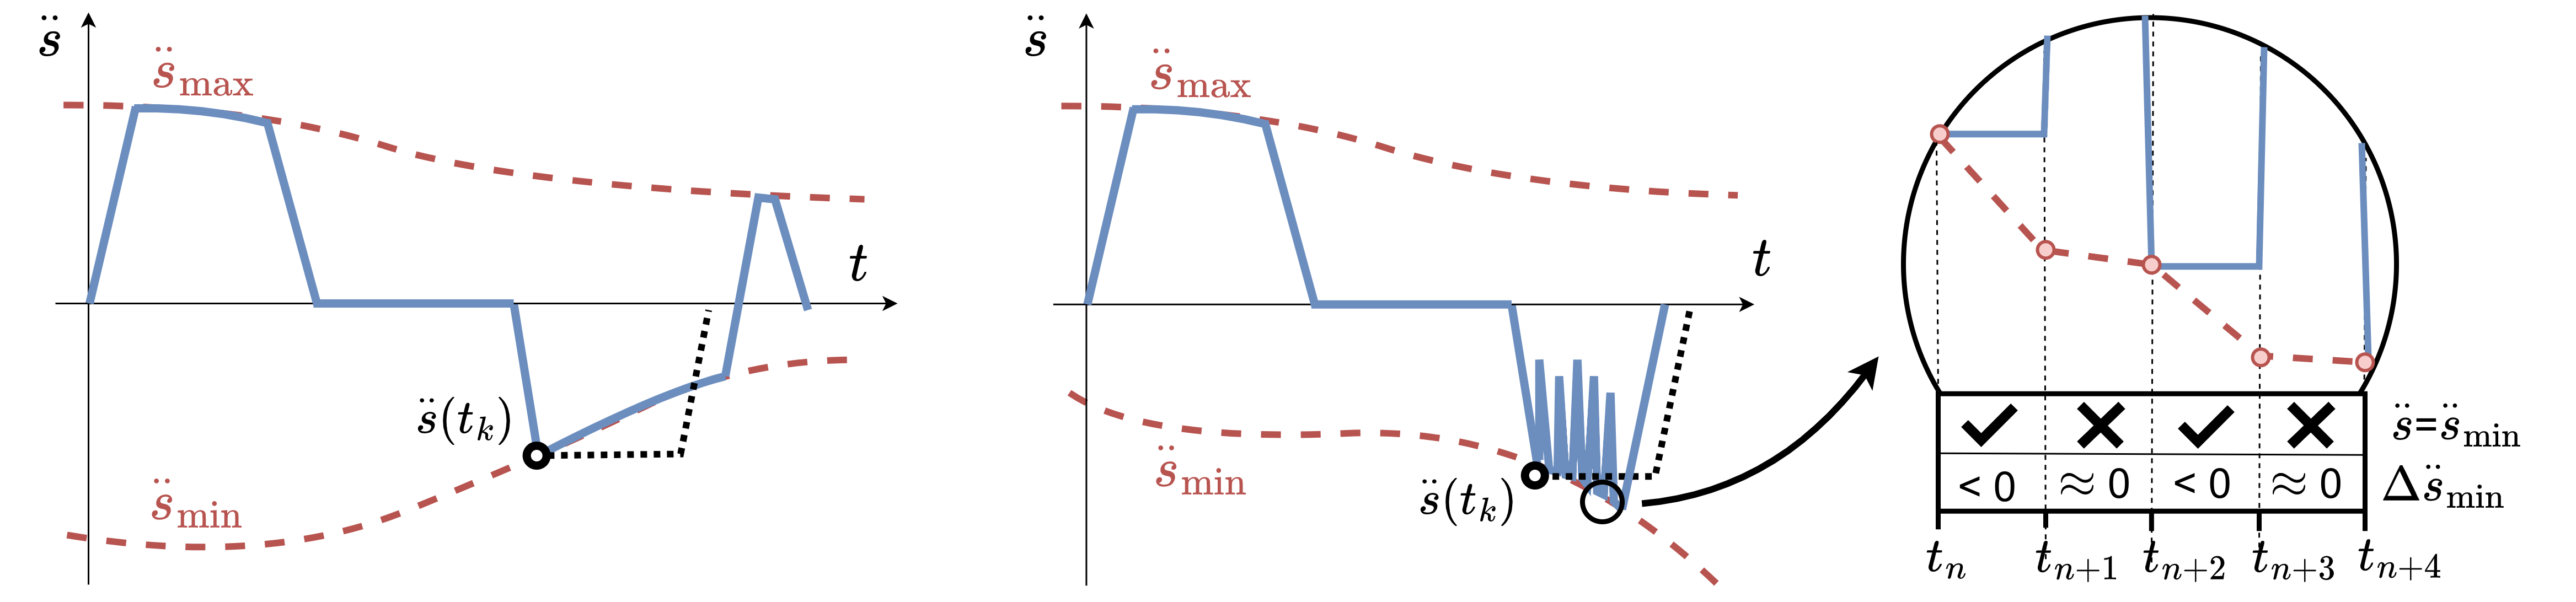
\includegraphics[width=\linewidth]{img/heuristics.png}
    \caption{Examples of negative effects that arise when considering robot's acceleration limits constant until the end of the trajectory. Figure on the left shows the effect of diminishing braking capacity towards the end of the trajectory, where the end result is an overshoot. The figure on the right shows the effect of augmenting braking capacity towards the end of the trajectory. Due to, in some cases, inverse proportional coupling between the robot's velocity $\dot{\bm{q}}$ and the braking capacity, more the robot brakes, more its velocity $\dot{\bm{q}}$ decreases and more the braking capacity increases. This effect produces an oscillatory behavior as showed in the zoomed view and the accompanying table. }
    \label{fig:overshoot_shema}
\end{figure}

The proposed approach adapts to the constant changes of the robot's motion capabilities by planning the new TAP trajectory at each time step $t_k$. For each planning iteration it considers constant robot's capabilities until the end of the trajectory. This assumption is reasonable as only the first step of each planned trajectory is used, in which the calculated robot's capabilities are valid. 
However, based on the prediction of robot's constant movement capacity the TAP planning decides the phase of the trajectory, when to stop accelerating and when to start braking. Therefore, in some cases, especially when robot's capacity changes significantly towards the end of the trajectory, TAP planning can produce oscillations and an overshoot due to the switching between the modes of braking and accelerating.

As shown on Figure \ref{fig:overshoot_shema}, there are two main scenarios that generate unwanted behavior, both related to the robot's deceleration (braking) capacity. 

\subsubsection{Decreasing braking capacity} When the robot's deceleration capacity decreases towards the end of the trajectory, left plot on Figure \ref{fig:overshoot_shema}, the planned trajectory will have an overshoot. Due to considering robot's capacity constant, robot's braking capacity is overestimated and when the TAP planning decides to start braking, at the time step $t_k$, it is already too late, the robot is not able to stop before it reaches the target position. 

This is an inherent challenge of real-time planning and cannot be solved without adding a degree of prediction of the robot's future capabilities. One such approach to mitigate the overshoot is to predict the robot's minimal braking capacity for the remaining cartesian path $P\left(s(t_i)\right)$ until the end of the trajectory $ t_i \in \left[t_k, T\right]$ and use this value for TAP planning.
\begin{equation}
    \ddot{s}_{min} = \max \left\{\ddot{s}_{min}(t_i)\right\} \quad t_i \in \left[t_k ,~ T\right]
\label{eq:minimal_braking_capacity}
\end{equation}
This approach in many cases results in more conservative trajectories as the robot's braking capacity is underestimated, but at the same time it guarantees the overshoot removal. As the robot's braking capacity depends on its joint configuration $\bm{q}$, finding the minimal braking capacity (\ref{eq:minimal_braking_capacity}) requires either knowing the exact robot's joint space path until the end of the trajectory, which is by definition not known, or finding all the possible joint configurations the robot can be in on the remaining path, which is very long and not practical for most real-time applications.

In this paper a sampling based approximation of (\ref{eq:minimal_braking_capacity}) is proposed based on sampling the remaining the path into $N$ cartesian posses $\mathcal{X}_i$. The most probable predictions joint space configurations $\bm{q}_i$ at each of the poses $\mathcal{X}_i$ is proposed to be found as the robot's inverse kinematics solution the closest to the current pose $\bm{q}_k$. Finally, the prediction of (\ref{eq:minimal_braking_capacity}) can be found as the minimal braking capacity among all the sampled ones $\ddot{s}_{i, min}$
\begin{equation}
    \ddot{s}_{min} = \max \left\{\ddot{s}_{0, min},~ \ldots,~ \ddot{s}_{N, min}\right \}
\end{equation}

\todo[inline]{I am not talking about how to decide which joint velocity $\dot{\bm{q}}_i$ to use!}

\subsubsection{Increasing braking capacity}
When the robot's breaking capacity increases along the trajectory, scenario shown on the right plot of Figure \ref{fig:overshoot_shema}, the proposed method can result in oscillatory behavior.  Due to considering robot's capacity constant, robot's braking capacity is underestimated and the decision of the TAP planning to start braking, at the time step $t_k$, comes too soon. In the next step $t_{k+1}$ the robot's breaking capacity increases which in term makes TAP planning stop braking. The repetitions of this sequence create the oscillations of the planed acceleration profile and produces jerky trajectories. 

The effect of these oscillations is greatly amplified as the robot's braking capacity $\ddot{s}_{min}$ is inverse proportional to the robot's current joint velocity $\dot{\bm{q}}_{k}$ through the bias term $\bm{a}_b = \dot{J}(\bm{q}_k,\dot{\bm{q}}_k)\dot{\bm{q}}_k$. Lowering the the joint velocity $\dot{\bm{q}}_{k}$, lowers the bias $\bm{a}_b$ and increases the braking capacity $\ddot{s}_{min}$. This effect creates a closed loop behavior, where more the robot brakes, more its braking capacity increases. 

In order to smooth the acceleration profile and reduce the effect of coupling introduced by the bias $\bm{a}_b$, a simple strategy is proposed which consists in down-sampling the TAP planning. Instead of planning the TAP trajectory in each time step $t_k$, the trajectory is planned with the time step $\Delta t_p$, while linearly interpolating the trajectory between the planning steps $t \in \left[t_k, t_k+\Delta t_p\right]$. 

\begin{equation}
    s(t) = s_k + \frac{s_{k+1}-s_k}{\Delta t_p}(t - t_k), \quad t \in \left[t_k, t_k + \Delta t_p\right]
\end{equation}
The same linear interpolation can be applied to the velocity $\dot{s}$ and acceleration $\ddot{s}$
\begin{equation}
\begin{split}
    \dot{s}(t) &= \dot{s}_k + \frac{\dot{s}_{k+1} - \dot{s}_{k}}{\Delta t_p}(t - t_k),\\
    \ddot{s}(t) &= \dot{s}_k + \frac{\ddot{s}_{k+1} - \ddot{s}_{k}}{\Delta t_p}(t - t_k)
\end{split}
\end{equation}
where $s_k$,$\dot{s}_k$ are $\ddot{s}_k$ are path position, velocity and acceleration in the current step $t_k$ and  $s_{k+1}$,$\dot{s}_{k+1}$ are $\ddot{s}_{k+1}$ are the their optimal values in the next planning step $t_{k+1}=t_k + \Delta t_p$ calculated by the TAP planning. 

% \todo[inline]{maybe stop here and in the experiments I say which filtering params we used.} 
\todo[inline]{discuss maybe a bit how/why this works, and that we consider robot's capacity static between the time steps $\Delta t_p$.
say also that this interpolation is an approximation and the longer the $\Delta t_p$ more it's wrong.} 


% \todo[inline]{
% Or use this approach.


% In order to smooth the acceleration profile and reduce the effect of coupling introduced by the bias $\bm{a}_b$, a simple strategy is proposed which consists in low pass filtering the bias term.
% \begin{equation}
%     \bm{a}^*_{k,b} = \alpha  \bm{a}_{k,b} +  (1-\alpha)  \bm{a}^*_{k-1,b}, \quad \alpha = \frac{T_s}{T_s + T_c}
% \end{equation}
% where $T_s$ is the sampling time of the trajectory planning and $T_c$ is the time constant of the filter corresponding to $T_c = 1/f_c$, where $f_c$ is the cutoff frequency of the filter. The new filtered bias $\bm{a}^*_{k,b}$ can then be used for determining the braking capacity $\ddot{s}_{k,min}$ as explained in the section \ref{ch:capacity_lp}. }




\section{Experimental setup}
\label{ch:setup}


All the experiments, both in simulation and in real world, are conducted on a Franka Emika Panda robot. The robot's kinematic limits in joint space and the Cartesian space are obtained from Franka Emika's official datasheet\cite{frankadata}.

\begin{table}[h!]
    \centering
 \caption{Franka Emika Panda robot joint space (JS) kinematic limits.}
    \begin{tabular}{c|ccc}
Joint & $\dot{\bm{q}}_{max}$ $[{rad}/{s}]$ & $\ddot{\bm{q}}_{max}$  $[{rad}/{s^2}]$ & $\dddot{\bm{q}}_{max}$   $[{rad}/{s^3}]$
\vspace{0.05cm}\\
\hline
 1 & 2.175 & 15 & 7500 \\
 2 & 2.175 & 7.5 & 3750 \\
 3 & 2.175 & 10 & 5000 \\
 4 & 2.175 & 12.5 & 6250 \\
 5 & 2.61 & 15 & 7500 \\
 6 & 2.61 & 20 & 10000 \\
 7 & 2.61 & 20 & 10000\\
\end{tabular}
    \label{tab:panda_limits_js}
\end{table}

\begin{table}[h]
\caption{Franka Emika Panda robot Cartesian Space (CS) limits.}
\label{table:franka_limits}
\centering
\begin{tabular}{c|ccc}
Limits & $\dot{\bm{x}}_{max}$ & $\ddot{\bm{x}}_{max}$ & $\dddot{\bm{x}}_{max}$ \\
\hline
Translation & 1.7 $m/s$ & 13 $m/s^2$  & 6500 $m/s^3$\\
Orientation & 2.5 $rad/s$ & 25 $rad/s^{2}$  & 12500 $rad/s^{3}$\\
\end{tabular}
\end{table}


The implementation of the TAP trajectory generator is based on the open-source library ruckig \cite{ruckig}, while the efficient LP solver used for real-time CS limit calculation is GLPK\cite{glpk}.

\subsection{Robot control architecture}
\label{ch:qp}

\begin{figure}[!tb]
    \centering
    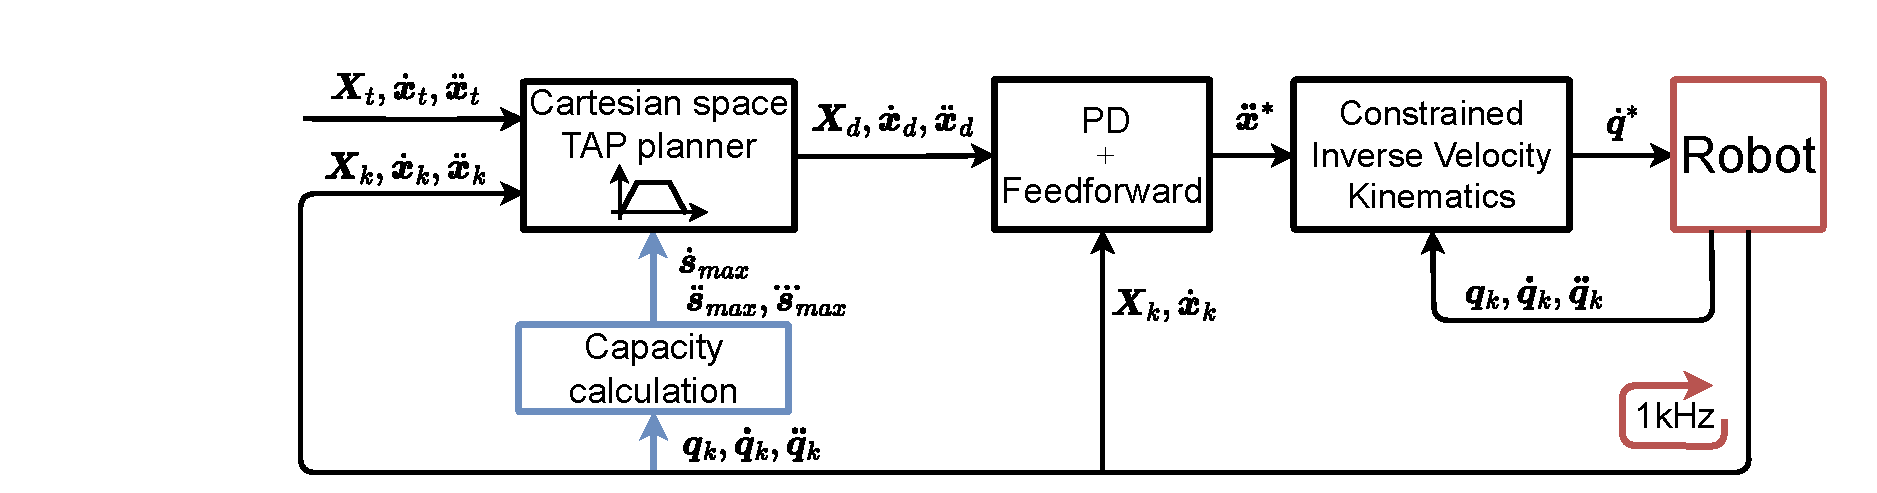
\includegraphics[width=\linewidth]{img/schema.pdf}
    \caption{Proposed method schematic overview in the context of the robot control, elements in blue present the extension of a standard CS based TAP planning.}
    \label{fig:schema}
\end{figure}

The schematic diagram of the proposed approach within the robot control paradigm is shown on Figure \ref{fig:schema}. Given the robot's current configuration $\bm{q}_k$, $\dot{\bm{q}}_k$, $\ddot{\bm{q}}_k$ in step $k$, the approach first determines the robot's current CS velocity $\dot{\bm{x}}_{max}$, acceleration $\ddot{\bm{x}}_{max}$ and jerk $\dddot{\bm{x}}_{max}$ limits. Then it calculates the new optimal trajectory, based on the TAP planning, given the robot's current Cartesian state $\mathcal{X}_k$,$\dot{\bm{x}}_k$,$\ddot{\bm{x}}_k$, the target state $\mathcal{X}_t$,$\dot{\bm{x}}_t$,$\ddot{\bm{x}}_t$ and the robot's kinematic limits $\dot{\bm{x}}_{max}$,$\ddot{\bm{x}}_{max}$,$\dddot{\bm{x}}_{max}$. 
Once the optimal TAP trajectory has been found, desired states $\mathcal{X}_{d}$,$\dot{\bm{x}}_d$,$\ddot{\bm{x}}_d$ are sent to the inverse velocity kinematics layer of the control architecture. 

In the case of this paper, robot control strategy for real-time Cartesian trajectory following is formulated as a Quadratic Program (QP) and solved in each control loop. As a secondary (regularization) task of the QP, the robot's redundant degrees of freedom are used to dampen the movement in the trajectory \textit{null-space} and keep the robot away from its joint limits.
\begin{equation}
\begin{split}
    \ddot{\bm{q}}_{opt} = \arg \min_{\ddot{\bm{q}}}& \quad || \dot{\bm{v}} - J_k\ddot{\bm{q}} - \dot{J}_k\dot{\bm{q}} ||^2 + \omega_r || \ddot{\bm{q}}_r - \ddot{\bm{q}} ||^2 \\
    \text{s.t.} \quad \ddot{\bm{q}} &\in [\ddot{\bm{q}}_{ub}, ~\ddot{\bm{q}}_{lb}]
\end{split}
\end{equation}
where the trajectory following  control law is formulated as a PD controller with a feed-forward term through the desired Cartesian acceleration $\dot{\bm{\nu}}^*$
\begin{equation}
\begin{split}
    \dot{\bm{\nu}}^* &= K_p \bm{e} + K_d(\dot{\bm{x}}_{d} - \dot{\bm{x}}_k) + \ddot{\bm{x}}_{d} \\
    \bm{e} &= \text{Ad}(\mathcal{X}_k) \log(\mathcal{X}_k^{-1}\mathcal{X}_{d})\\
\end{split}
\end{equation}
$\mathcal{X}_d$,$\dot{\bm{x}}_d$,$\ddot{\bm{x}}_d$ are the desired Cartesian pose, velocity and acceleration in the next step $k+1$ , $\mathcal{X}_{k}$ and $\dot{\bm{x}}_{k}$ are the measured Cartesian pose and velocity in current step $k$. $K_p,K_d\in \mathbf{R}^m$ are diagonal matrices containing the proportional and derivative gains. Vector $\bm{e}$ is the Cartesian pose error expressed in the world frame. The regularization task is expressed through the joint acceleration $\ddot{\bm{q}}_r$
\begin{equation}
    \ddot{\bm{q}}_r = k_{rp}(\bm{q}_{r} - \bm{q}) - k_{rd}\dot{\bm{q}}
\end{equation}
where $k_{rp}$ and $k_{rd}$ are scalar gains and $\bm{q}_{r}$ is the initial robot pose close to the center of all the joint ranges. The bounds of each of joint accelerations $\ddot{{q}}_{i,ub}$, $\ddot{{q}}_{i,lb}$ are calculated in a way to guarantee that the joint jerk $\dddot{\bm{q}}$, velocity $\dot{\bm{q}}$ and position $\bm{q}$ in the horizon $\delta t$ respect their limits. 
% \begin{equation}
%     \begin{split}
%         \ddot{{q}}_{i,ub} = \min \Big\{ &\ddot{{q}}_{i,k} + \dddot{q}_{i,max}\delta t, \\
%         &\ddot{{q}}_{i,max},\\ 
%         &\frac{1}{\delta  t}(\dot{{q}}_{i,max} - \dot{{q}}_{i,k}), \\ 
%         &\frac{2}{\delta  t^2}({{q}}_{i,max} - {{q}}_{i,k} - \dot{{q}}_{i,k}\delta  t )\Big\}  \\
%     \end{split}\label{eq:qp_limits}
% \end{equation}
\begin{equation}
\begin{split}
    &\ddot{{q}}_{i,ub} = \min  \Big\{ \ddot{{q}}_{i,k} + \dddot{q}_{i,max}\delta t, 
    \ddot{{q}}_{i,max}, \; ..\\
    &\frac{1}{\delta  t}(\dot{{q}}_{i,max} - \dot{{q}}_{i,k}),  
    \frac{2}{\delta  t^2}({{q}}_{i,max} - {{q}}_{i,k} - \dot{{q}}_{i,k}\delta  t )\Big\}  
\end{split}\label{eq:qp_limits}
\end{equation}
where the horizon $\delta t$ has to be chosen long enough to ensure constraints compatibility without leading to conservative behaviour\cite{Prete2018}. Equation (\ref{eq:qp_limits}) shows the upper bound expression, the lower bound calculation is equivalent, and is obtained by substituting \textit{min} for \textit{max} and maximizing instead of minimizing.

Robot is controlled using the joint velocity commands which are calculated using an Euler backward numerical integration
\begin{equation}
\dot{\bm{q}}^*_{k+1} = \dot{\bm{q}}^*_{k} +  \ddot{\bm{q}}_{opt}\Delta t  
\end{equation}

In the experiments, the PD controller gains used are $K_p=\text{diag}([170.0, 170.0, 170.0, 100.0, 100.0, 100.0])$ and $K_d=\text{diag}([50.0, 50.0, 50.0, 30.0, 30.0, 30.0])$. The secondary task gains used are $k_{rp}=5 s^{-2}$ and $k_{rd}=2\sqrt{k_{rd}}s^{-1}$, while secondary task weight is $\omega_r=1e^{-5}$. The horizon $\delta t$ is chosen to be 15ms. 


\subsection{Compensating the overshoot and oscillation effects}

As proposed in section \ref{ch:heuristics}, in order to avoid the overshoot due to the decreasing robot's braking capabilities and the oscillations induced by the coupling bias $\bm{a}_b$, two compensation strategies are used in the experiments
\begin{itemize}
    \item predicting robot's future braking capability
    \item down-sampling the TAP planning  
\end{itemize}

\begin{figure}[!tb]
    \centering
    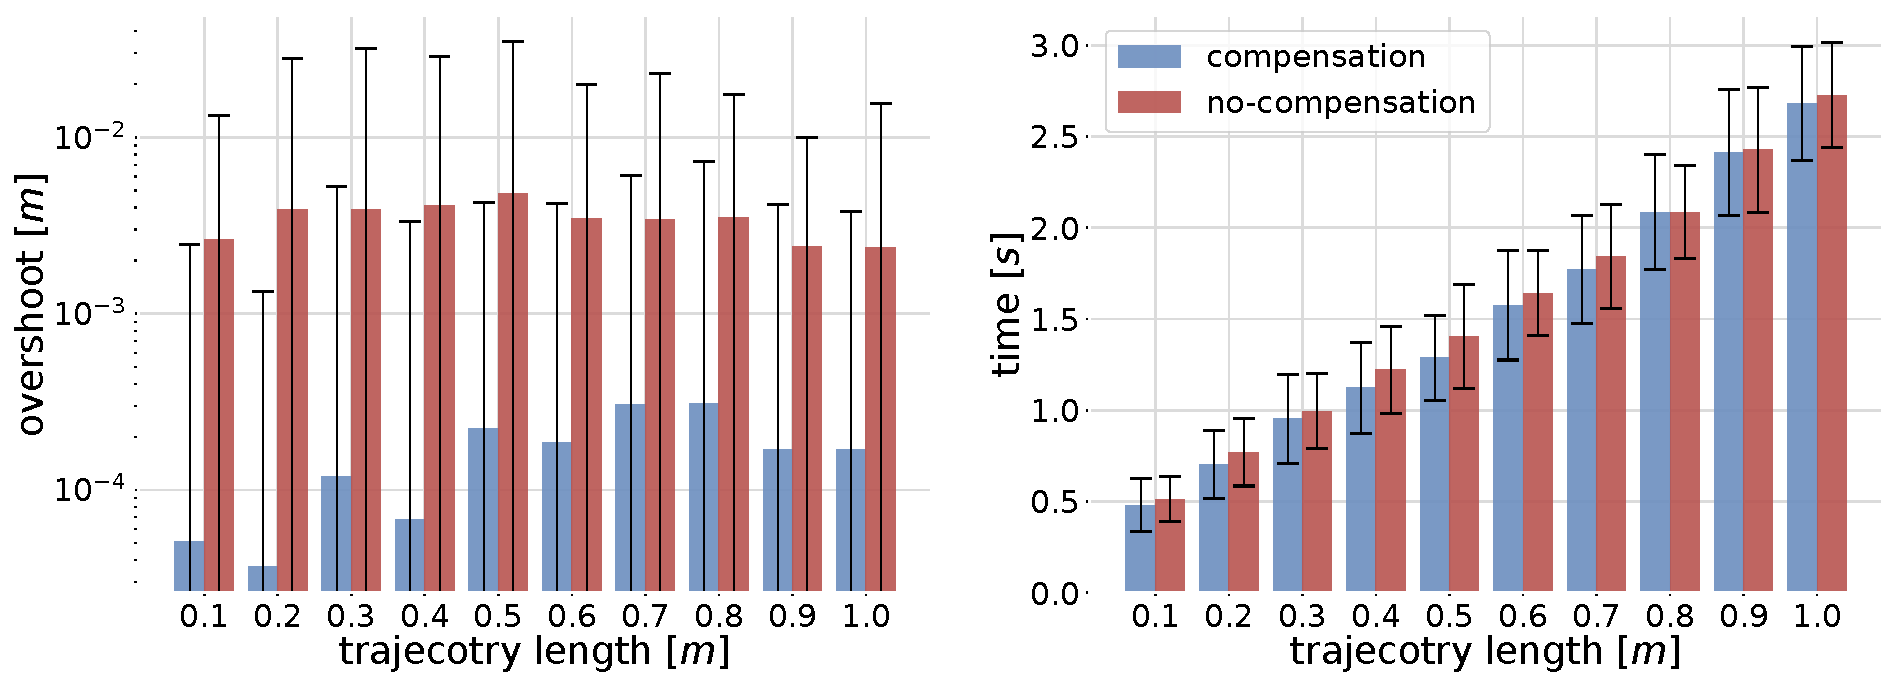
\includegraphics[width=\linewidth]{img/compensation_comp.pdf}
    \caption{Plots showing the comparison of the average overshoot (left) and average execution time (right) of the proposed method with and without overshoot compensation. For each length ranging from $d=0.1$ to $1m$, means and variances are calculated over 100 random trajectories. }
    \label{fig:compensatiopn_comp}
\end{figure}

\subsubsection{Predicting robot's braking capacity} on the remaining trajectory is implemented using the sampling method. Where the remaining CS path is sampled with $N$ positions and robot's braking capacity is calculated for each one of them. Finally the minimal braking capacity among the sampled ones is used for TAP planning. In the experiments the remaining trajectory is sampled with $N=2$ points, corresponding to the current position $\mathcal{X}_k$ in the time step $t_k$ and the final position at the end of the trajectory $\mathcal{X}_T$. Joint configuration $\bm{q}_T$ at the $\mathcal{X}_T$ is found as the inverse kinematics solution the closest to the current configuration $\bm{q}_k$ and the joint velocity $\dot{\bm{q}}_T$ and acceleration $\ddot{\bm{q}}_T$ are considered to be $0$ as the robot will come to a stop at the target $\mathcal{X}_T$. Finally the braking capacity used for TAP planning in the step $t_k$ is the minimum of the two
\begin{equation}
    \ddot{s}_{min} = \max\left\{\ddot{s}_{k,min}, \ddot{s}_{T,min}\right\}
\end{equation}

Figure \ref{fig:compensatiopn_comp} presents a comparison between the proposed method's performance with and without overshoot compensation. To evaluate the methods, 1000 random translation trajectories (random fixed orientation) were generated in the robot's workspace, ranging in length from $d\!=\!10cm$ to $d\!=\!1m$. The overshoot and execution time were recorded for each trajectory. The results indicate that the proposed method with overshoot compensation significantly reduces the expected overshoot compared to the method without compensation, going from $3mm$ average overshoot to $0.1mm$. Moreover, the compensation strategy does not have a negative impact on the trajectory execution time. On the contrary, it slightly reduces the average execution time, as shown in the figure.

\todo[inline]{calculated the end pose braking capacity only once}

\subsubsection{TAP planning down-sampling} has been implemented as suggested in section \ref{ch:heuristics}, where the TAP planning was executed each $\Delta t_{p}\!=\!10ms$, each $10$ steps of the control algorithm. In order to find an optimal down-sampling time an empirical study has been conducted for 100 random trajectories with lengths $d=40cm$, $60cm$ and $80cm$ in the robots workspace. Four down sampling times were compared $\Delta t_p =1ms$, $5ms$, $10ms$ and $50ms$. For each executed trajectory the maximal deviation from the path and the Cartesian jerk variance is evaluated. 
\begin{figure}[!t]
    \centering
    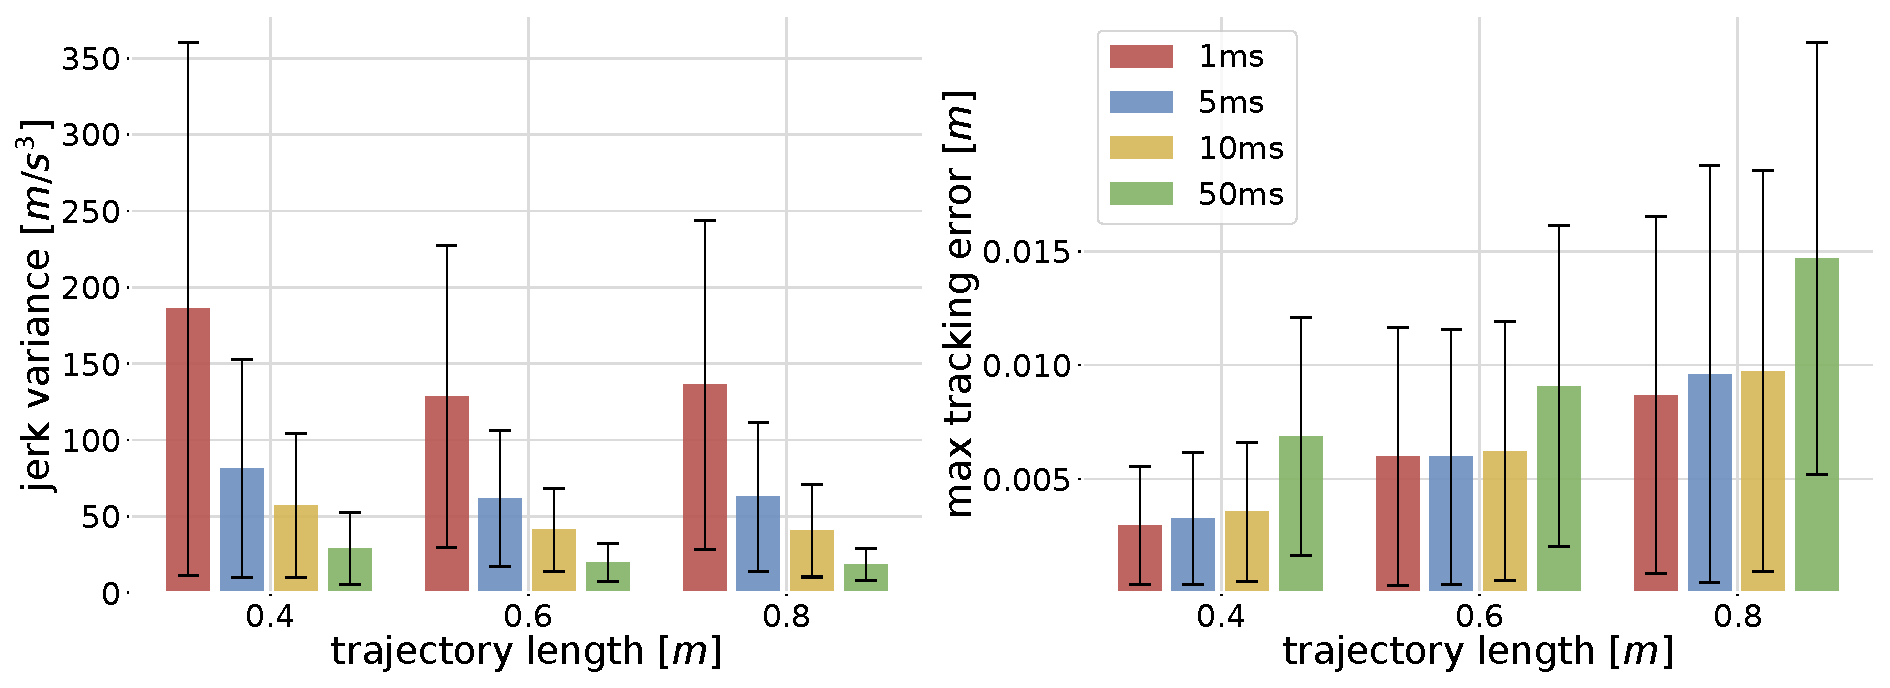
\includegraphics[width=\linewidth]{img/compensation_comp_oscillations.pdf}
    \caption{Plots showing the comparison of the jerk variance(left) and following error (right) of the proposed method with and without oscillation compensation, for trajectory lengths $d=0.4$, $0.6$ and $0.8m$. Means and variances are calculated over 100 random trajectories. }
    \label{fig:compensatiopn_comp_oscillations}
\end{figure}

Figure \ref{fig:compensatiopn_comp_oscillations} demonstrates an inverse proportionality between the down sampling time and the jerk variance. Additionally, it reveals that as the planning time step $\Delta t_p$ increases, there is a corresponding increase in the deviation from the desired path. This implies that a trade-off must be made, and the optimal planning step $\Delta t_p$ appears to fall between the range of $5ms$ to $10ms$.

\section{Comparative study}
\label{ch:comp_study}
A simulation based comparative study is conducted to evaluate the performance of the proposed method against the well known time-optimal planning algorithms. The proposed algorithm is first compared to the state of the art time-optimal joint space planning method called TOPP-RA \cite{Pham2018}. Furthermore the proposed algorithm is compared against the TAP planning with fixed Cartesian space limits provided by the manufacturer.

Both comparative studies are implemented in python
using open-source implementations of TOPP-RA \cite{Pham2018} and TAP planning (Ruckig library \cite{ruckig}). 
Robot rigid body dynamics simulation was implemented using the open-source library Pinocchio \cite{pinocchio2021}. 
All the code used for the experiments is open-source and can be found on gitlab\footnote{https://gitlab.inria.fr/auctus-team/people/antunskuric/papers/tap_capacity}.

\subsection{Benchmarking against time-optimal JS planning}

\begin{figure}[!t]
    \centering
    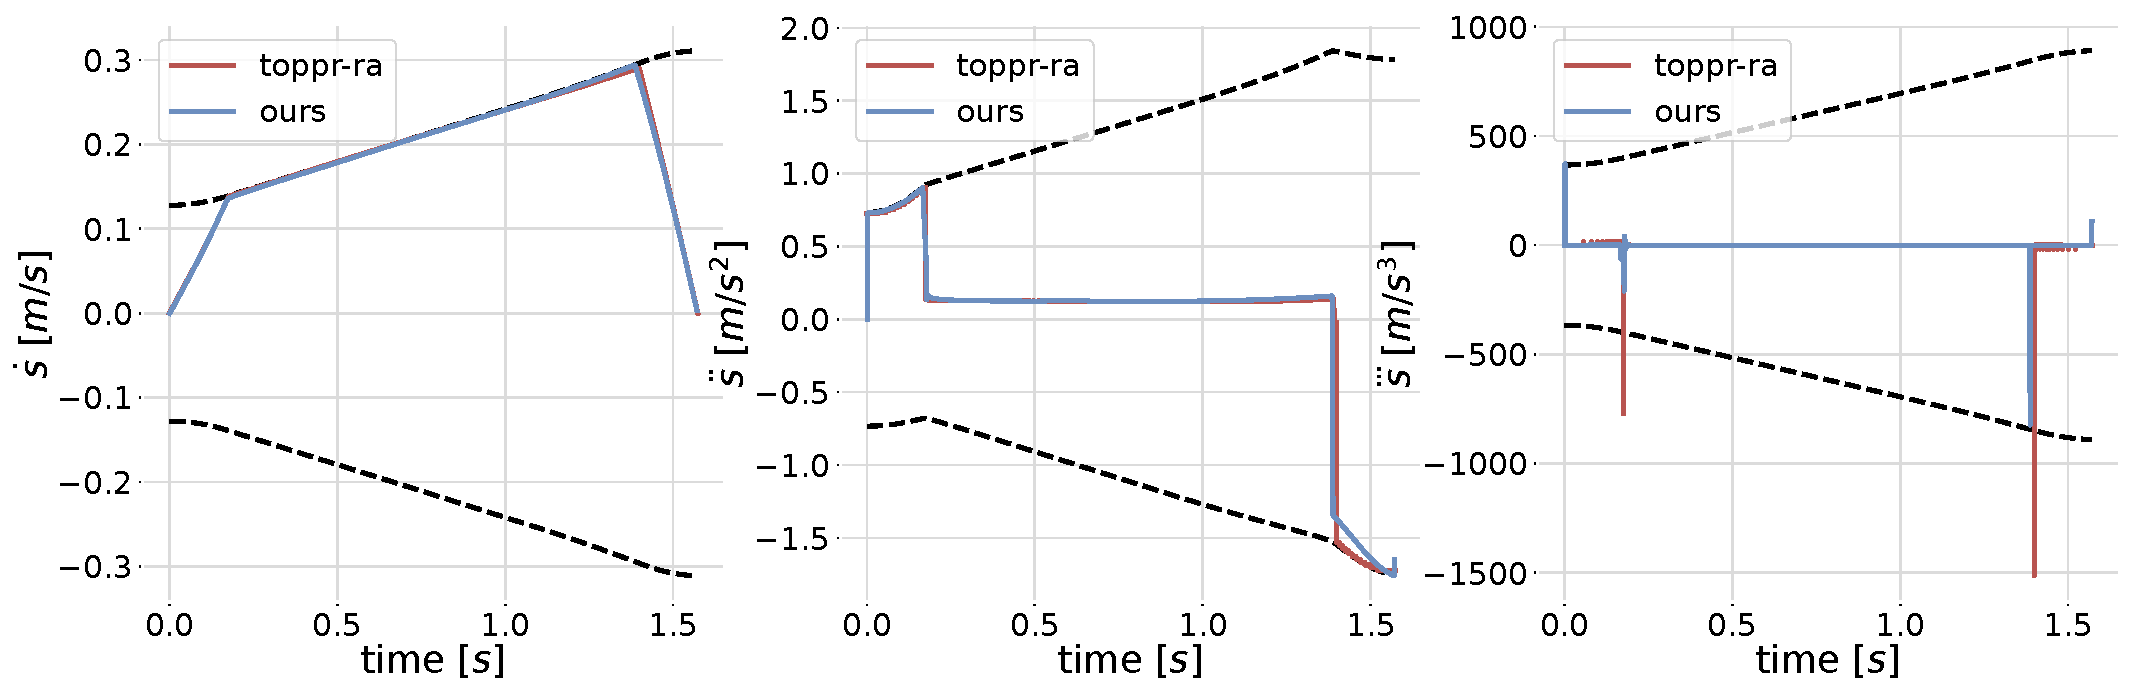
\includegraphics[width=\linewidth]{img/ruckig_toppra_comp1679478306.pdf}
    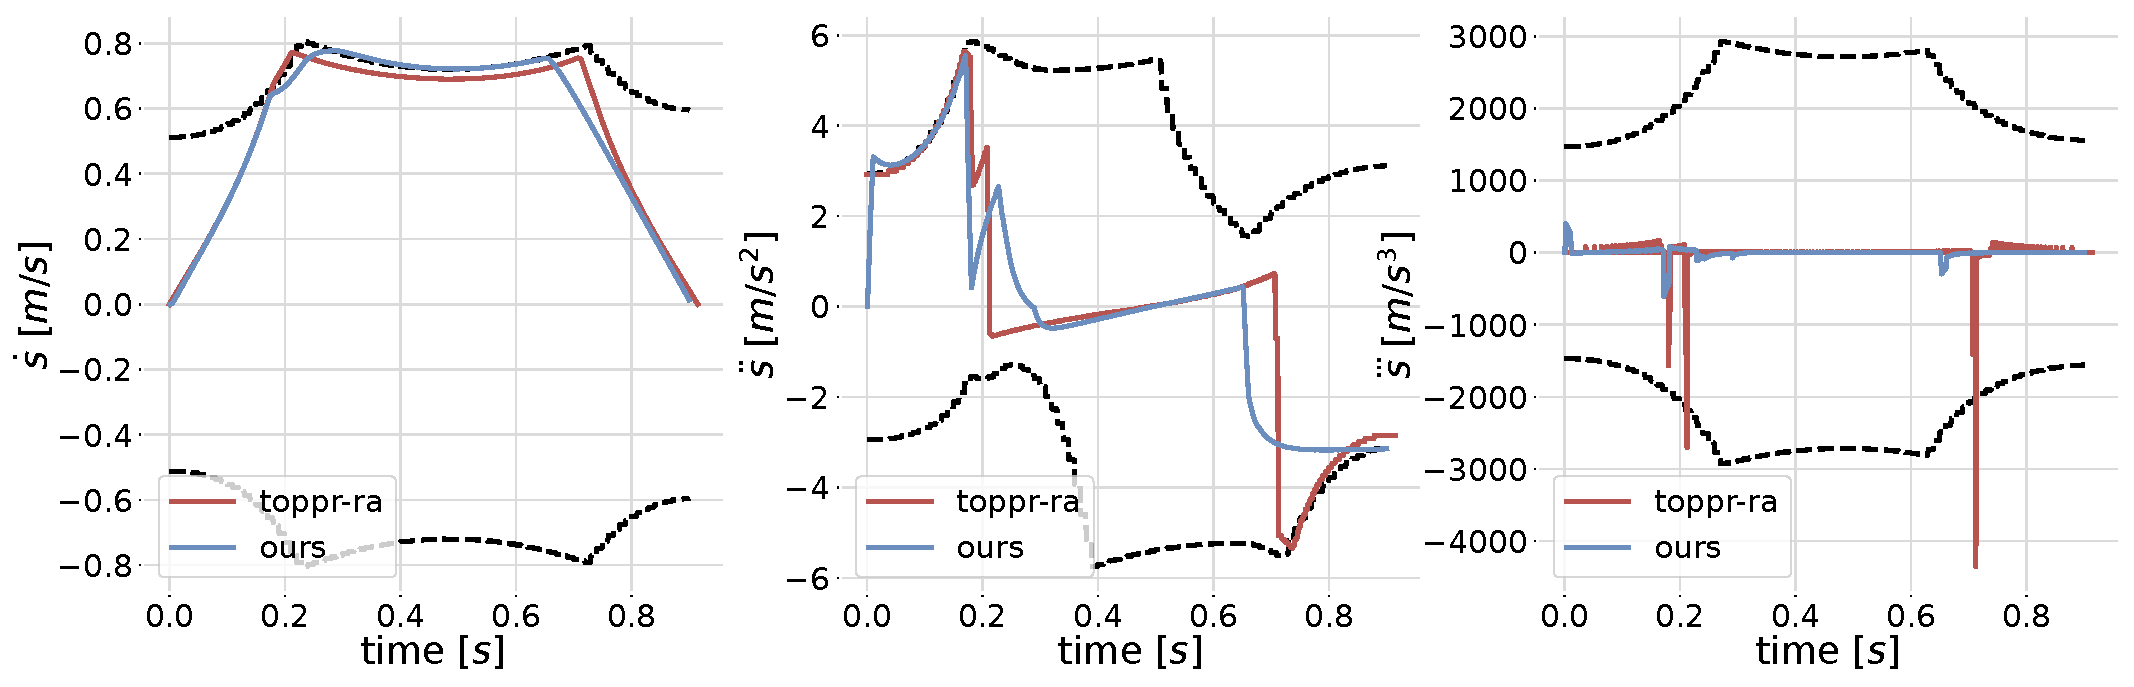
\includegraphics[width=\linewidth]{img/ruckig_toppra_comp1681374566.pdf}
    \caption{The plots show the comparison of the path velocity, acceleration and jerk, generated by the proposed approach (blue) and TOPP-RA(red), for two different trajectories (up and down). }
    \label{fig:comparison_trajectory}
\end{figure}

In order to evaluate the performance of the trajectories found and executed by the proposed Cartesian space planning approach, it is benchmarked against the state-of-the art time-optimal joint space planning algorithm TOPP-RA \cite{Pham2018}. TOPP-RA takes in consideration the robot's joint space velocity and acceleration limits and plans for the minimum time joint space trajectories.
Both algorithms are run on a set of 1000 random straight line trajectories (with random fixed orientation), ranging in length from $d=10cm$ to $1m$. The goal of this experiment being to compare the generated trajectory profiles of TOPP-RA and the proposed approach as well as their execution times, in order to asses the tome optimally of the proposed real-time planning approach. 

TOPP-RA's limitation however is that it cannot deal with Cartesian space trajectories directly and it requires an additional step of finding the joint space path corresponding to the Cartesian space path.  For TOPP-RA, the full joint space path is determined by sampling the Cartesian path $P(s)$ into the set of waypoints $\mathcal{X}_{w,i}$ and finding the inverse kinematic solution $\bm{q}_{w,i}$ for each one of them. To ensure the JS path continuity, the inverse kinematics solution $\bm{q}_{w,n+1}$ at the waypoint $\mathcal{X}_{w,n+1}$ is taken as the one closest to the joint configuration $\bm{q}_{w,n}$ in the previous waypoint $\mathcal{X}_{w,n}$.

Both approaches are tested using 50\% of the robot's JS velocity, acceleration and jerk capacity $\alpha_v\!=\!\alpha_a\!=\!\alpha_j = 0.5$. The distance between the waypoints used in this paper is $5cm$. 

\todo[inline]{argue about the 5cm waypoint and 50\% capacity.}


\subsubsection*{Results} Comparison of the planned velocity, acceleration and jerk profiles for two trajectories are shown on Figure \ref{fig:comparison_trajectory}. It can be seen that both methods find similar time profiles for all the path variables, indicating the effectiveness of the proposed approach. Moreover, even though TOPP-RA plans entirely in joint space its Cartesian space trajectory respects the CS velocity and acceleration limits calculated by the proposed method, demonstrating the accuracy of limit calculations. Additionally, TOPP-RA does not limit the jerk which can be seen on the jerk plots in Figure \ref{fig:comparison_trajectory}.

Additionally, the influence of the overshoot compensation strategy can be observed in the second (bottom) trajectory. The proposed approach starts braking earlier and does not use the full braking capacity of the robot. The resulting trajectory does not have an overshoot, even though the robot's braking capacity drops significantly towards the end of the trajectory. This demonstrates the effectiveness of the proposed strategy in reducing overshoot while not significantly increasing the execution time.

\todo[inline]{Something like that}
The trajectory execution time comparison is presented in Figure \ref{fig:comparison_time}. The figure shows that the proposed method has a comparable execution time for all tested trajectory lengths. Interestingly, for lengths over $40cm$, our approach is even faster than TOPP-RA. This can be attributed to the fact that our method takes a different joint space (JS) path than TOPP-RA, which in some cases might be more optimal than the one calculated in advance. 
\textcolor{red}{This effect is more present for longer trajectories where taking the joint space path the closest to the initial joint configuration might not be the most optimal criteria. }


\todo[inline]{say that this is not planned and that this happens more for the long trajectories because the chance that the toppra's JS trajectory is not optimal is higher for them than for the shorter ones.}

\begin{figure}[!t]
    \centering
    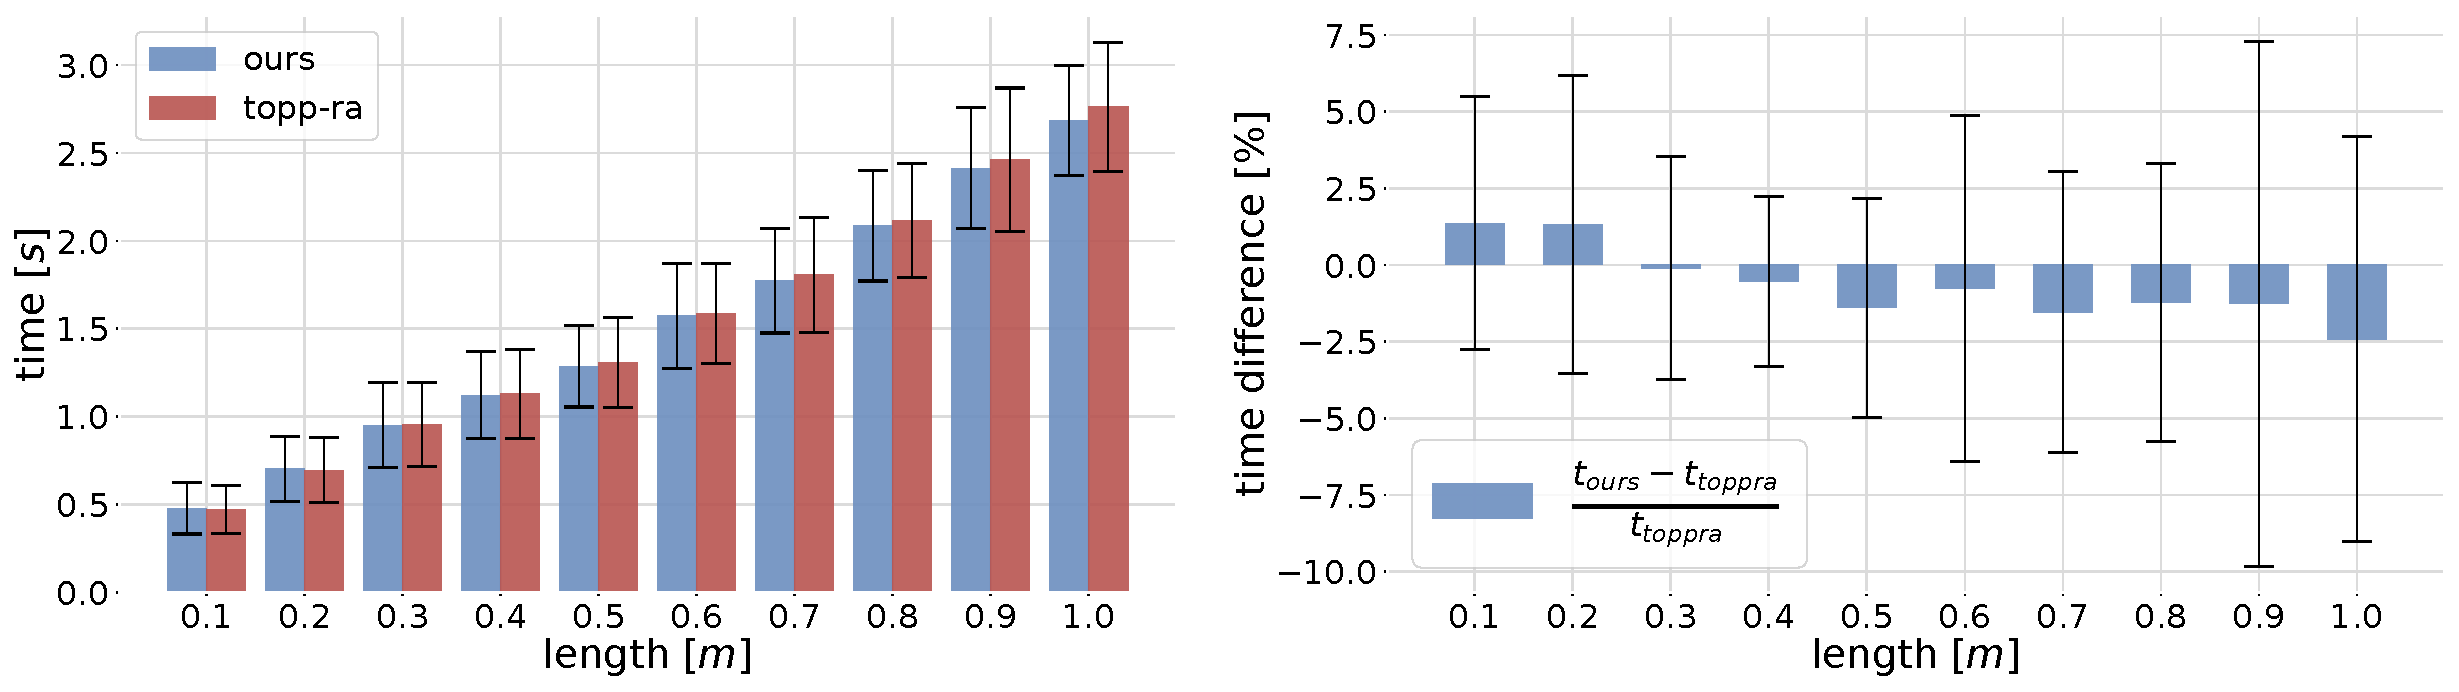
\includegraphics[width=\linewidth]{img/toppra_ruckig_time_comp.pdf}
    \caption{Plots showing the comparison of the trajectory execution time of the proposed method with TOPP-RA, for trajectory lengths ranging from $d=0.1$ to $1m$. Left graph shows the comparison of the execution time, while the graph on the right shows the difference in execution time in a form of percentage. Means and variances are calculated over 100 random trajectories.}
    \label{fig:comparison_time}
\end{figure}
\subsection{Benchmarking against time-optimal  CS planning}



\begin{figure*}[!t]
    \centering
    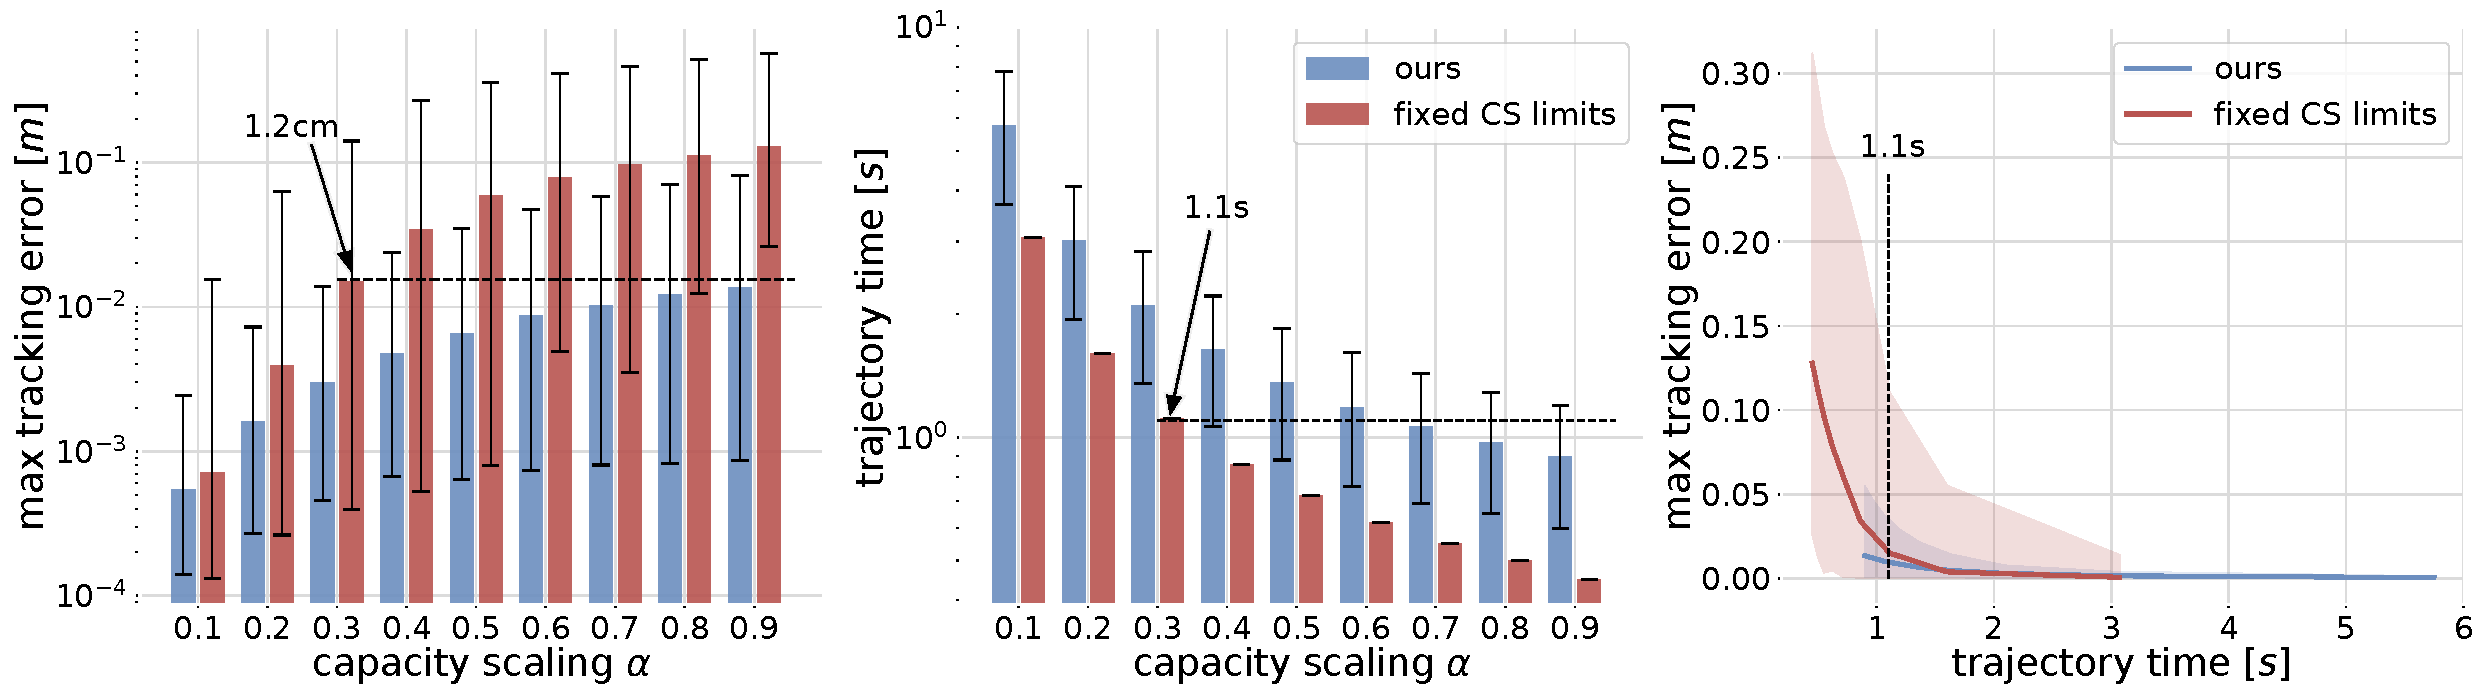
\includegraphics[width=\linewidth]{img/comparison_fixed_cs.pdf}
    \caption{Result of the benchmarking experiment comparing the fixed CS planning approach (red) to the proposed method (blue). The graph on the left shows comparison of the max tracking error with respect to the ratio of the capacity $\alpha$ used while the graph in the middle shows the trajectory execution time comparison. The graph on the right unites the two graphs on the left in order to show the relation of the trajectory execution time against the max tracking error. Means and variances are calculated on 100 random robot trajectories. }
    \label{fig:comp_fixed_cs}
\end{figure*}
The proposed adaptive approach is further compared to the standard TAP trajectory planning using fixed Cartesian kinematic limits. The Cartesian space limits for the Franka Emika panda robot are taken from the standard datasheet \cite{frankadata}, as given in Table \ref{table:franka_limits}.

The approaches are compared over 100 random robot straight line trajectories (with random fixed orientation), in the robot's workspace, with a fixed length of $d=50cm$. The performance of the two approaches is compared for different scaling levels $\alpha$, starting at 10\% ($\alpha$=0.1) of robot's capacity and going to 90\% ($\alpha$=0.9). The scaling strategy is chosen to be equal for velocity, acceleration and jerk $\alpha\!=\!\alpha_v\!=\!\alpha_a\!=\!\alpha_j$. 



The implementation of the TAP trajectory generator for both approaches is done using the open-source library ruckig \cite{ruckig}. The robot control strategy implemented for trajectory following is the same for both approaches as detailed in the section \ref{ch:qp}.

\subsubsection*{Results} In Figure \ref{fig:comp_fixed_cs}, the results of a comparative study between the proposed method and the TAP planning method with fixed CS limits are presented. Both methods show a linear relationship between the tracking error and the ratio of capacity used ($\alpha$), however the proposed approach has a significantly lower mean error and variance for the same $\alpha$. This can be attributed, in part, to the overestimated CS limits (Table \ref{table:franka_limits}) provided by the manufacturer for the Panda robot, see Figure \ref{fig:comp_cube_poly}.


Figure \ref{fig:comp_fixed_cs} further shows that using 30\% of the manufacturer's CS limits (i.e., $\alpha$=0.3) results in a tracking error of around 1.2cm, which is higher than any of the mean errors achieved by the proposed method for all tested values of $\alpha$.
While for $\alpha$=0.3, the fixed CS planning has the execution time of 1.1 seconds, the proposed method has lower execution time for all $\alpha\geq0.7$. 
\textcolor{red}{These results therefore confirm that when it comes to planning for highly dynamical trajectories, taking in consideration robot's true movement capacity results in faster and more precise movements. }




% \begin{figure*}[!t]
%     \centering
%     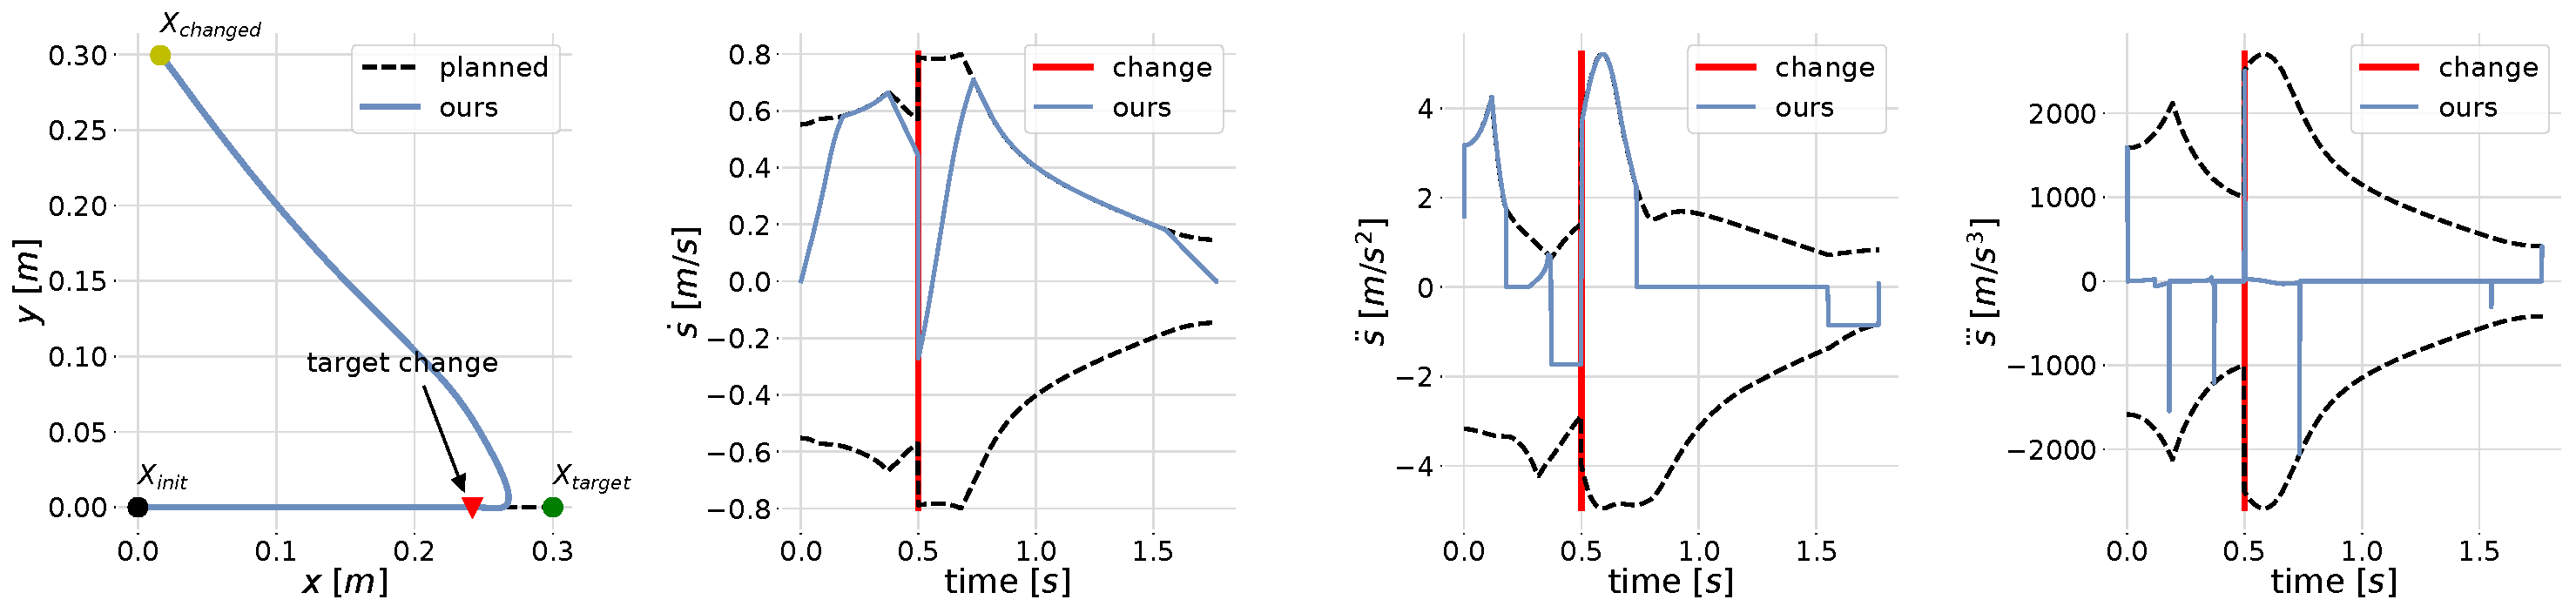
\includegraphics[width=\linewidth]{img/ruckig_plots_change_aio1680176621.pdf}
%     \caption{Write this}
%     \label{fig:change target}
% \end{figure*}



\section{Mockup experiment: Adaptive (Collaborative) waste sorting}
\label{ch:experiment_mockup}
% \begin{figure*}[!t]
%     \centering
%     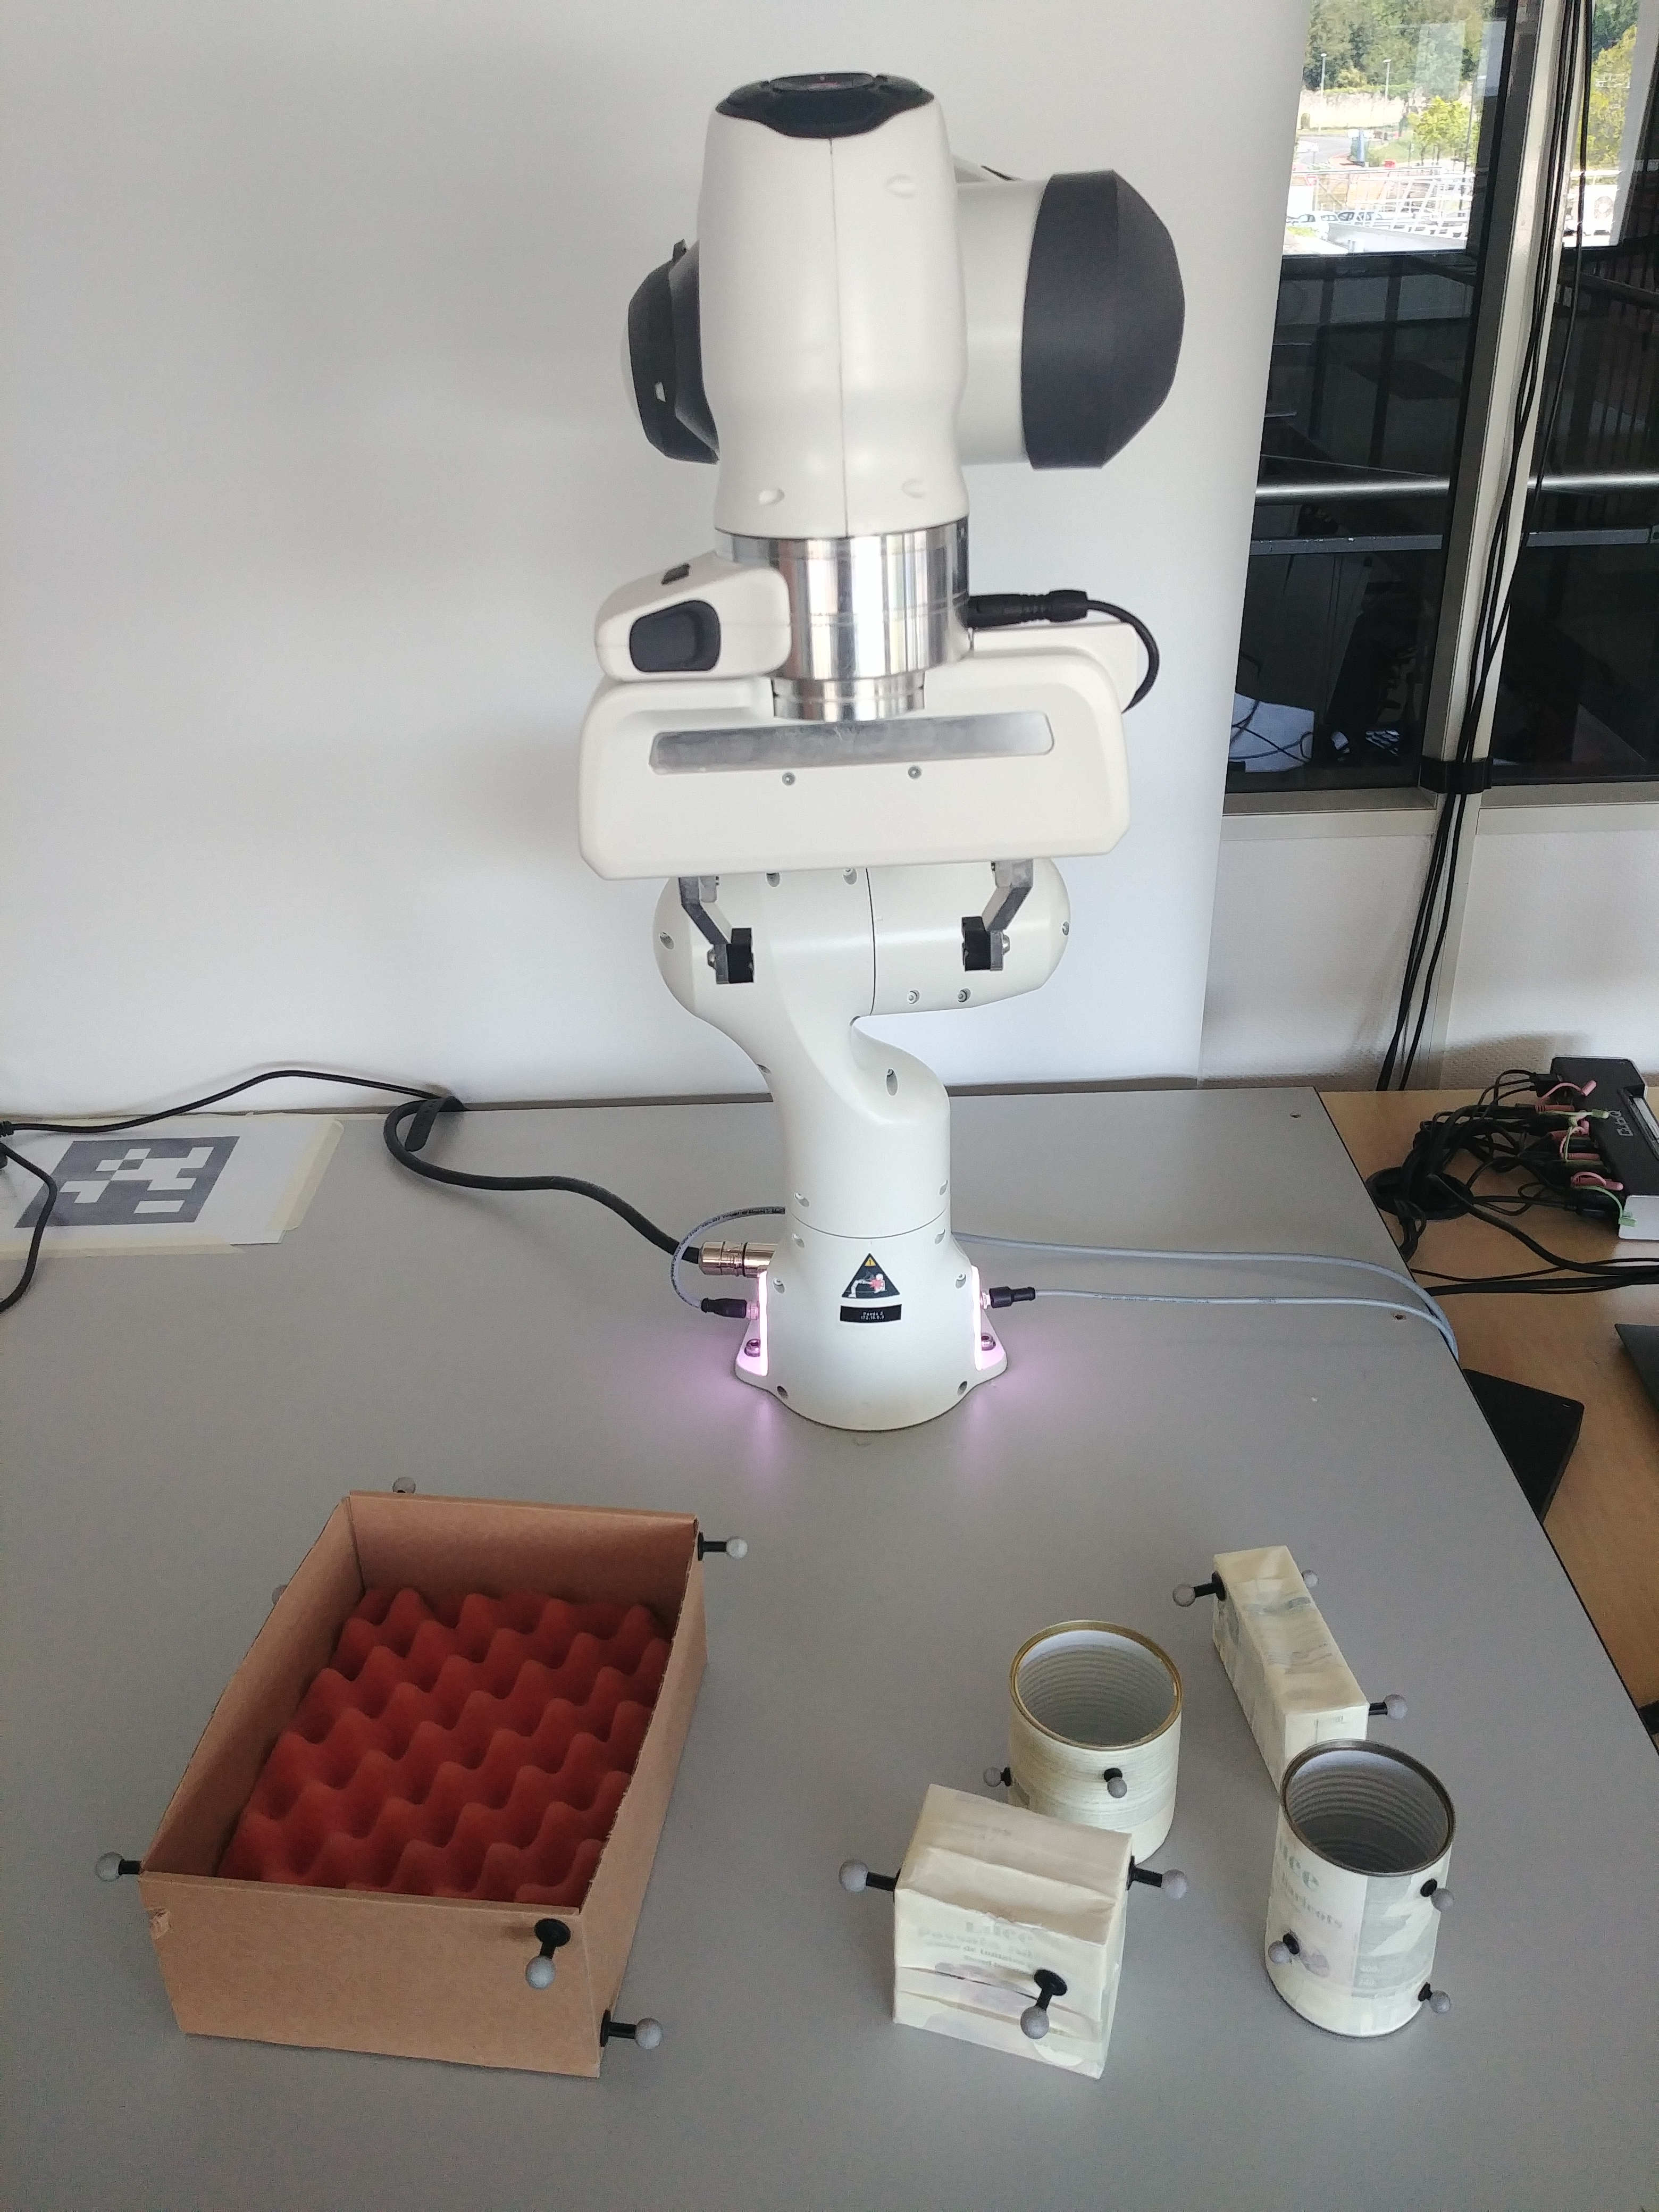
\includegraphics[width=0.26\linewidth]{img/setup.jpg}   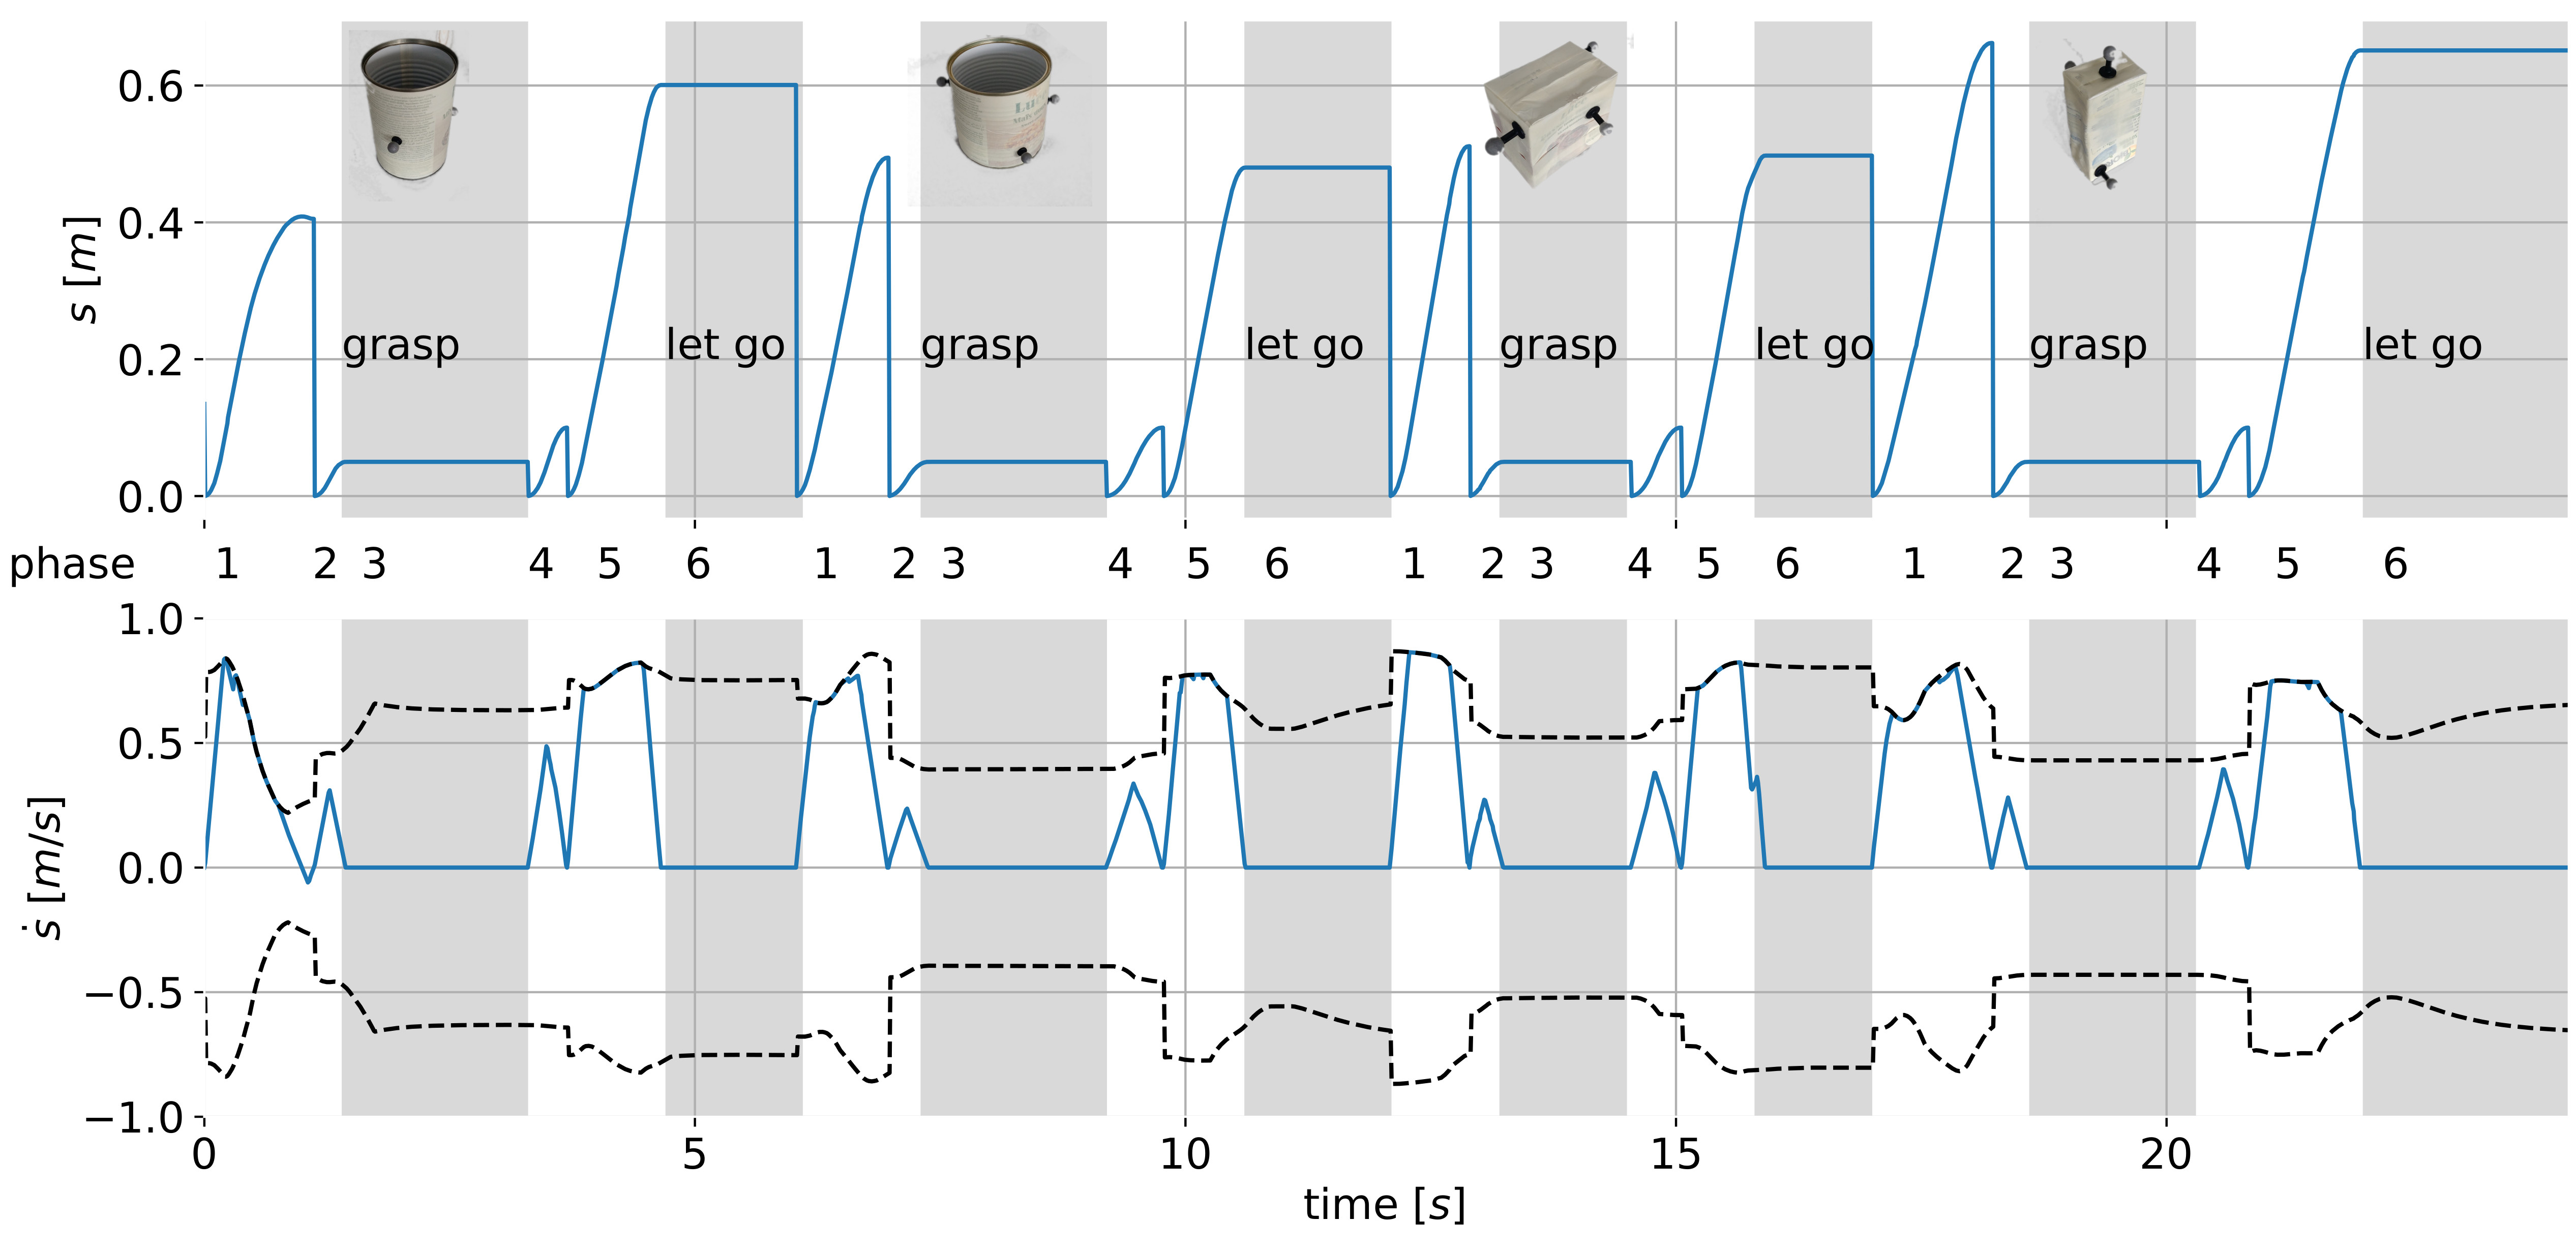
\includegraphics[width=0.73\linewidth]{img/experiment_main.jpg}
%     \caption{Write this}
%     \label{fig:setup}
% \end{figure*}
\begin{figure*}[!t]
    \centering
    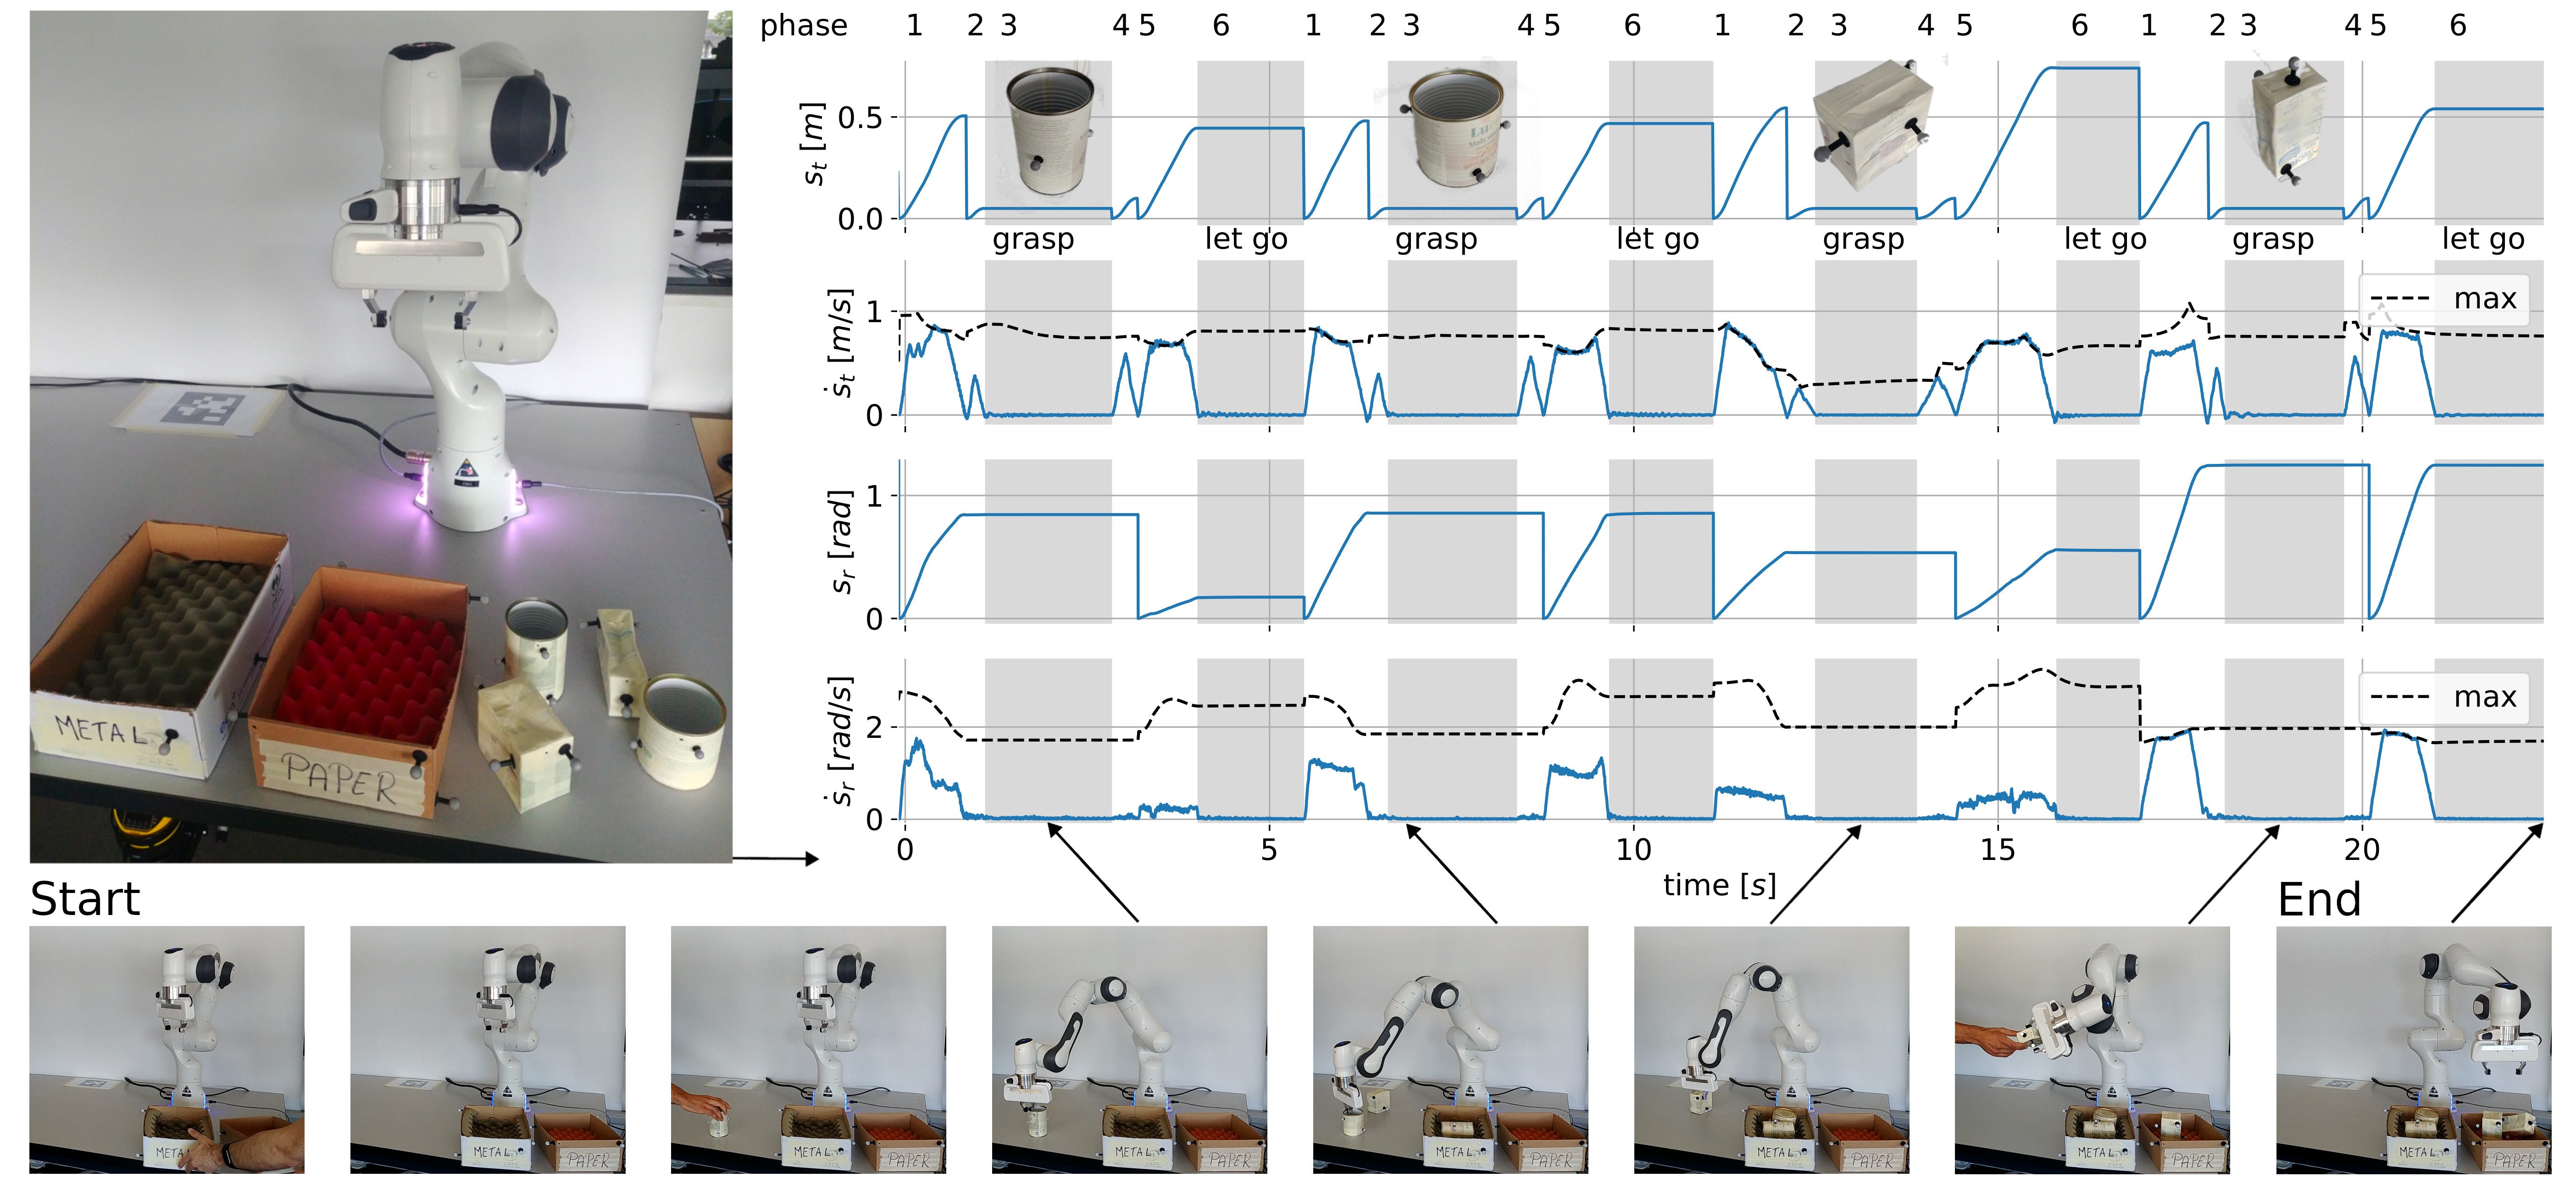
\includegraphics[width=\linewidth]{img/experiment_main_v2.3.jpg}   
    \caption{Figure on the left shows the experimental setup for the mockup waste sorting experiment. Franka Emika Panda robot is uses as well as six objects two cans and two cartons and two sorting bins, all tracked in real time using Motion capture system Optitrack. The images on the bottom show some key moments of the experiment, while the plot (up right) shows the time evolution of the real-time executed trajectories. The plot shows the position $s_t$ and orientation $s_r$ path evolution in time as well as translation $\dot{s}_t$ and rotation $\dot{s}_r$ velocity on the path and their calculated maximal values (dotted lines).  In the experiment, the operator first brings the sorting bins to the robot workstation, then introduces the waste objects to the robot with unknown positions and orientations. Robot plans and executes in real-time the trajectories necessary in order to place, as fast as possible, the objects into the appropriate sorting bin.}
    \label{fig:setup}
\end{figure*}

Waste sorting is an important ecological issue that can benefit from the use of robotics and computer vision technologies in order to greatly improve the waste processing efficiency and the volume \cite{Koskinopoulou2021}. However, waste sorting is a highly dynamic and unstructured environment, presenting a challenge for robot movement generation.
To be viable, waste sorting robots need to be able to operate at high speeds, where they use pick-and-place or pick-and-toss \cite{Hassan2022} techniques to sort the waste in different material groups.

Several robotic solutions have been proposed in the literature to address waste sorting tasks \cite{SARC2019}, such as \textit{Zenrobotics Fast picker}\footnote{https://zenrobotics.com/de/} or \textit{SELMA}\footnote{https://www.opteknik.se} . However, these solutions are based on expensive industrial robots and are only viable for large scale recycling facilities.

In this work, we propose a mocap interactive (collaborative) scenario for waste sorting that leverages the proposed real-time trajectory planning method in order to create fast and adaptable robot movement. 

In the experiment, a human operator is introducing the different waste items on the sorting workstation, where the robot is placed. The human can introduce the waste in any time and order, as well as modify their position and orientation on the table and the position and the orientation of the sorting bucket. The robot's job is to pick all the waste items and place them in the sorting buckets as fast as possible.

Waste items (two cans and two cartons) are tracked in real-time using a motion capture system \textit{Optitrack} as well as the buckets. In order to efficiently and robustly sort the waste, object manipulation procedure is divided in 6 phases.
\begin{enumerate}
    \item Position the gripper 5cm above the object with the appropriate orientation
    \item Lower the gripper to the object
    \item Close the gripper
    \item Rise the object 10cm
    \item Transport the object to the appropriate bucket
    \item Release the object
\end{enumerate}

Robot control architecture, as described in chapter \ref{ch:qp}, and the proposed real-time planning approach are implemented in 
programming language c++, using \textit{Robot Operating System} (ROS) framework, and run in real-time at the frequency of 1kHz. For this experiment, 60\% of robot's capacity has been used ($\alpha$=0.6) in order to keep the tracking error under 1cm, as shown on Figure \ref{fig:comp_fixed_cs}.

Figure \ref{fig:setup} shows the time evolution of one run of the experiment. The plot shows the evolution of the translation $s_t$ and orientation $s_r$ in time as well as their respective velocities  $\dot{s}_t$,  $\dot{s}_r$. The gray areas show the moments in time where the gripper was closing or opening in order to grasp or let go of an object. Several moments during the experiment run are shown on the images around the plot.

The experiment starts with the human operator bringing the sorting bins (metal and paper) and placing them in the robot's workspace. Then the operator introduces the objects (sometimes multiple at a time) on the robot's workstation table, while the robot plans and executes the necessary trajectories in real time, in order to place the objects in appropriate sorting bins. Objects' and bins' positions and orientations are not known in advance and can change in real-time. 

The velocity $\dot{s}_t$, $\dot{s}_r$ plots show that the proposed approach was able to follow robot's changing capacity and produce motions with maximal possible reachable velocities. It can also be seen that for different trajectories executed, either translation velocity $\dot{s}_t$ or rotation velocity $\dot{s}_r$ is maximised, The reason why they are not both exploited is because the translation and orientation is synchronised in order for the robot to reach both target position and orientation at the same time.

The adaptability of the proposed approach is further demonstrated as the final waste item is handed over to the robot, where the robot grasps the object from the operator's hand. 

\todo[inline]{
figure out what else to conclude here. Maybe add how this approach could be used for safety.
}

\section{Discussion on the limitations}
\label{ch:discussion}

\todo[inline]{
too honest?
}
As shown in previous sections, the proposed trajectory planning approach has many benefits over the classic time-optimal approaches. It is capable of efficiently exploiting robot's true movement capacity while being reactive at the same time and allowing changes in the trajectory on the fly. However, the proposed approach has several limitations.

The main limitation of the proposed approach is its assumption that the Cartesian path can be represented using using only one variable $s(t)$ (or two $s_t(t),s_r(t)$ in case of both translation and orientation). 
This assumption enables transforming polytope based robot's capacity metrics (\ref{eq:limits_poly}) to the interval ranges of path variables (\ref{eq:s_limits}). These ranges can then be efficiently calculated in real-time and used with the standard trajectory planning algorithms such as TAP.  
The consequence of such assumption is that the planned trajectory can guarantee respecting the calculated limits only in the trajectory direction, which is reasonable for straight line trajectories. However, if trajectory is not a straight lines or if it is a straight lines but the target position suddenly changes during the trajectory execution, the proposed approach will not be able to guarantee respecting the robot's limits in the directions orthogonal to the trajectory. In order to overcome this effect, trajectory planning algorithms that would be able to use the polytope representation of path constraints (\ref{eq:limits_poly}) would be needed. However, such planning algorithms are still not available, to the best of our knowledge, and therefore represent a a promising future research direction.

Different consequence of this issue is that the proposed approach assumes translation and orientation paths independent. However, the limits on velocity, acceleration and jerk of both paths are not independent, as both translation and rotation are generated by the same robot actuators with the limits (\ref{eq:kin_limits}). The true limits on the path variables $s_t$ and $s_r$ would have a form of a polytope. A way to avoid this issue could be to define the path in Lie space, where the rotation and translation could be represented in one path variable. However, in that case, the robot would no longer move in straight lines in Cartesian space. In order to minimise the coupling effect between the rotation and translation, in the context of this paper, translation limits are calculated while considering constant rotation velocity, while rotation limits are calculated considering constant translation velocity. 

Another limitation of the proposed approach is the assumption of the constant robot's capacity for every planning iteration. As described in the section \ref{ch:heuristics}, this can lead to certain negative effects such as an overshoot or oscillations.  In order to overcome this issue, instead of considering only instantaneous robot's capacity for each trajectory generation execution, it would be necessary to predict the robot's kinematic capacity along the remaining trajectory. This is a challenging research topic which results might be applied not just in TAP planning techniques but also to the optimal control methods such as Model predictive control (MPC).  

Finally, the robot's joint space kinematic limits (\ref{eq:kin_limits}) are considered constant in time, which is generally not the case.
These limits will depend on the robot's actuation limits $\bm{\tau}$ and different dynamical and gravitational effects acting on the robot, as well of the robot's joint state $\{\bm{q},\dot{\bm{q}}\}$. Therefore, for highly dynamical robot's movements, the available actuation capacity of the robot might reduce certain of the limits (\ref{eq:kin_limits}). Therefore, the integration of the robot's actuation limits $\bm{\tau}$ could make the proposed approach more robust and it is a promising direction for future research. 

% \todo[inline]{
% \begin{itemize}
%     \item 
% say something about straight lines also maybe?
% \item waypoints and singularities
% \item some positives like safety applications (velocity modulation)
% \end{itemize}
% }

\section{Conclusion}

\todo[inline]{too long but more or less everythig is here.}

In this paper a new real-time Cartesian space trajectory planning algorithm is presented capable of fully exploiting robot's movement capacity. The proposed method leverages the efficient approach for projecting robot's joint space constraints in the trajectory direction, in order to evaluate the robot's velocity, acceleration and jerk limits in real-time. These limits are then used to plan the time-optimal Trapezoidal acceleration profile (TAP) trajectory for the remaining trajectory at each step of the trajectory execution. The proposed approach is able, in addition to the robot's actuation limits, to take in consideration additional task and the environment specific constraints, for example by modulating the robot's velocity when the operator is in vicinity in order to enforce his safety \cite{smu}.

The proposed method has been compared with the state of the art time-optimal joint space planning method called TOPP-RA. The results of the comparison show that the proposed method has a comparable trajectory execution time as TOPP-RA even though it is planning in real-time as opposed in advance optimisation done by TOPP-RA.
Furthermore, the proposed method is compared with the Cartesian space TAP planning considering constant Cartesian space limits given by the manufacturer. The results show than the proposed method exploits better robot's movement capacity and at the same time has lower tracking error. 

Finally, a mockup experiment is proposed presenting an application of the proposed method in collaborative waste sorting context. The human operator introduces different waste items on the collaborative workstation with unknown position and orientation and the robot uses the proposed method to plan the time-efficient trajectories in order to put all the waste items to the sorting bins.
